\documentclass[
 paper=A4,pagesize=automedia,fontsize=12pt,
 BCOR=15mm,DIV=22,
 twoside,headinclude,footinclude=false,
 english,fleqn,             % fleqn = linksbündige Ausrichtung von Formeln
 bibtotocnumbered,          % Literaturverz. im Inhaltsverz. eintragen
 liststotoc,                % Abbildungsverz. im Inhaltsverz. eintragen
 listsleft,                 % Abbildungsverz. an der längsten Nummer ausrichten
 pointlessnumbers,          % kein Punkt nach Überschriftsnummerierung
 cleardoublepage=empty      % Vakatseiten ohne Paginierung
]{scrbook}
\setlength\parindent{0em}

% Kodierung, Schrift und Sprache auswählen
\usepackage[utf8]{inputenc}
\usepackage[T1]{fontenc}
\usepackage[english]{babel}
% damit man Text aus dem PDF korrekt rauskopieren kann
\usepackage{cmap}
% Layout: Kopf-/Fußzeilen, anderthalbfacher Zeilenabstand
\usepackage{scrlayer-scrpage} \pagestyle{scrheadings}
                      \clearscrheadfoot
                      \ihead{\headmark}\ohead{\pagemark}
                      \automark[subsection]{section}
                      \setheadsepline{0.5pt}
\usepackage{setspace} \onehalfspacing
\usepackage{enumitem} \setlist{itemsep=0pt}
\deffootnote{1em}{1em}{\textsuperscript{\thefootnotemark }}
% clickable references
\usepackage{hyperref}
% Grafiken, Tabellen, Mathematikumgebungen
\usepackage[dvipsnames]{xcolor}
\usepackage{graphicx}
\usepackage{svg}
%\hypersetup{
%	colorlinks,
%	linkcolor={PineGreen},
%	citecolor={cyan!80!black},
%	urlcolor={blue!80!black}
%}
\usepackage{wrapfig}
\hypersetup{hidelinks}
\usepackage{tabularx, booktabs, makecell} \renewcommand{\arraystretch}{1.2}
\usepackage{amsmath,amsfonts,amssymb}
% Darstellung von Fließumgebungen
\usepackage{flafter,afterpage}
\usepackage[section]{placeins}
\usepackage[margin=8mm,font=small,labelfont=bf,format=plain]{caption}
\usepackage[margin=8mm,font=small,labelfont=bf,format=plain]{subcaption}
\usepackage{multicol}
\numberwithin{equation}{chapter}
\numberwithin{figure}{chapter}
\numberwithin{table}{chapter}

%%%%%%%%%%%%%%%%%%%%%%%%%%%%%%%%%%%%%%%%%%%%%%%%%%%%%%%%%%%%%%%%%%%%%%%%%%%%%%%%
% Ab hier ist Platz für eigene Ergänzungen (Pakete, Befehle, etc.)

% Dieses Paket liefert den Blindtext, der als Platzhalter in den Beispieldateien steht.
% Das kannst Du also entfernen, wenn Du den Blindtext nicht mehr brauchst.
\usepackage{lipsum}

\begin{document}



% Titelpageseite
\begin{titlepage}
 \begin{tabularx}{\linewidth}{X}
  
\includegraphics[width=6cm]{TU_Logo_SW} \\\hline\hline

  \vspace{4.5em}

  \begin{singlespace}\begin{center}\bfseries\Huge
  
  KZM on Si(1, 0, 0) Surface
  
  \end{center}\end{singlespace}

  \vspace{5.5em}

  \begin{singlespace}\begin{center}\large
   Master-Arbeit \\ zur Erlangung des Hochschulgrades \\ 
   Master of Science \\ 
   im Master-Studiengang Physik
  \end{center}\end{singlespace}\medskip

  \begin{center}vorgelegt von\end{center}
  \begin{center}
   {\large Andreas Weitzel} \\ geboren am 10.08.1999 in Fulda
  \end{center}\medskip

  \begin{singlespace}\begin{center}\large
   Institut für Theoretische Physik \\
   Fakultät Physik \\
   Bereich Mathematik und Naturwissenschaften \\
   Technische Universität Dresden \\ 2023
  \end{center}\end{singlespace}
 \end{tabularx}
\end{titlepage}


% Gutachterseite
\thispagestyle{empty}\vspace*{48em}

Eingereicht am xx.~Monat~20xx\vspace{1.5em}
\par{\large\begin{tabular}{ll}
 1. Gutachter: & Prof.~Dr.~XX \\
 2. Gutachter: & Prof.~Dr.~YY \\
\end{tabular}}


% Abstractseite
\newpage
\begin{center}\large\bfseries Summary\end{center}


Abstract \\ 
English: \\

\vspace{20em}
Abstract \\ 
Deutsch \\
 
 
% Inhaltsverzeichnis

%\cleardoublepage
\tableofcontents



% Hauptteil
\mainmatter
\chapter{Introduction}
\section{Motivation}
		Silicon has probably shaped our age like no other element and is responsible for large parts of the revolution humanity went through in the last couple of decades. It is a basic building block of our age, which is not without reason sometimes referred to as the silicon age. This is because of silicons semiconducting properties that are made use of in transistors and integrated circuit chips used in all our everyday electronic devices like smartphones and computers. More specific, Silicon is used in wafers, which are substrates for integrated circuits. Integrated circuits are just sets of smaller, basic electronic building blocks like transistors. Processors, GPUs, Random Access Memory 
	
	The surface is semiconducting \cite{himpsel1979photoemission, uhrberg1981experimental, handa1989plasma}


\chapter{The Si(0,0,1) Surface} \label{Section::Silicon}
	\section{Surface Reconstruction}
	Below a temperature of $T =	1687~\text{K}$ silicon crystallizes in a diamond cubic crystal structure \autoref{Fig::SiliconDiamond} with a lattice constant of $a =	5.431~\text{\AA} $ \cite{tiesinga2021codata}. When cutting this crystal structure along the (001) plane, the resulting system exhibits a surface reconstruction. Surface atoms are left with two dangling bonds. One of those dangling bonds can be invested into forming a dimer with the neighboring Si atom in (110) direction \cite{chadi1979atomic}, which leads to a large reduction of surface energy of $2~\text{eV}$ per dimer \cite{ramstad1995theoretical}.
	\begin{figure}[htp]
		\centering
		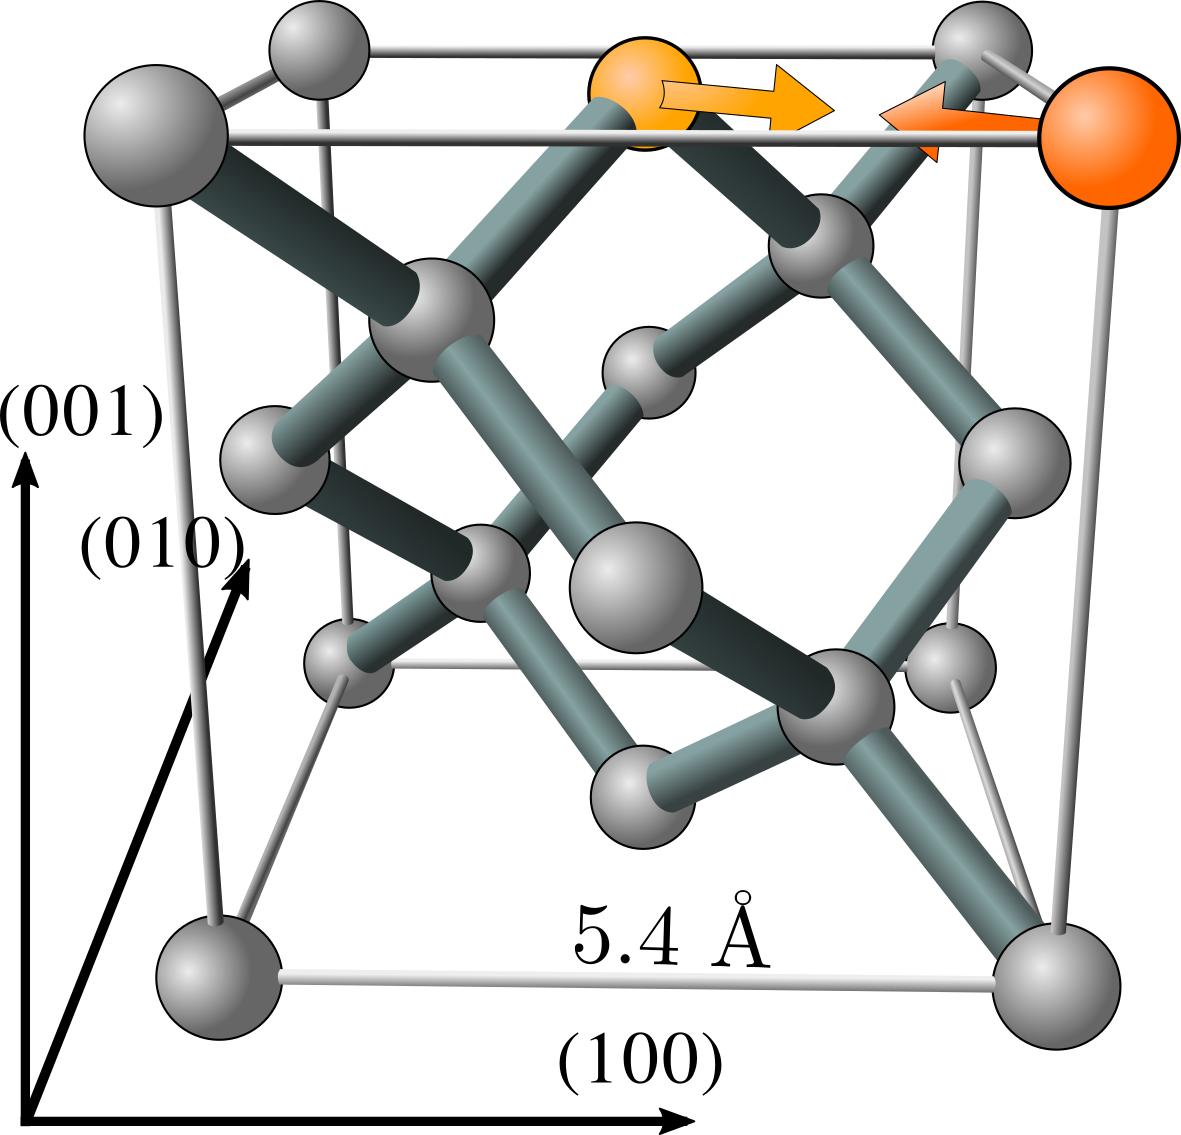
\includegraphics[width=0.7\linewidth]{graphics/Sili.png}
		\caption{The crystalline structure of Si in its solid state is shown. The orange colored atoms form a dimer when cutting the diamond structure along the (001) plane. The arrows on the left are normal to their corresponding planes. (TODO cite origin from wikipedia, mark your alterations)}
		\label{Fig::SiliconDiamond}
	\end{figure}
	
	The resulting dimers can further reduce their energy by vertical buckling. The dimers tilt to an angle of about $\approx 18^\circ$, which lowers the surface energy by another $0.2~\text{eV}$ per dimer. The buckling comes with a charge transfer of $\approx0.1 e$  \cite{brand2023critical, landemark1992core} and the resulting coulomb interaction leads to an alternating buckling of the dimers like shown in \autoref{c(4x2)}. The surface reconstruction with the lowest energy was through theoretical \cite{ramstad1995theoretical} and experimental \cite{brand2023critical} methods found to be the c(4x2) reconstruction as it minimizes the electrostatic interaction energy as well as the surface stress. 
	\begin{figure}[htb]
		\begin{subfigure}{0.5\textwidth}
			\centering
			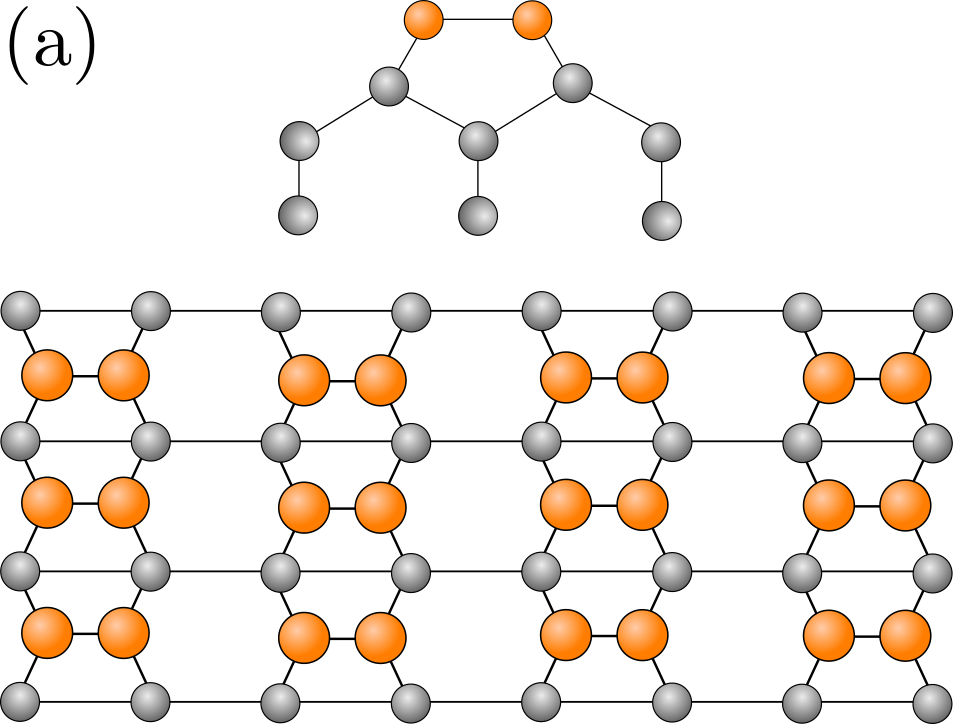
\includegraphics[width=0.8\textwidth]{graphics/p(2x1)-sym.png}
			\caption{The formation of dimers results in the symmetric p(2x1) reconstruction and saves a large amount of $2~\text{eV}$ per dimer compared to the ideal p(1x1) structure.}
			\label{p(2x1)-symmetric}
		\end{subfigure}
		\begin{subfigure}{0.5\textwidth}
		\centering
		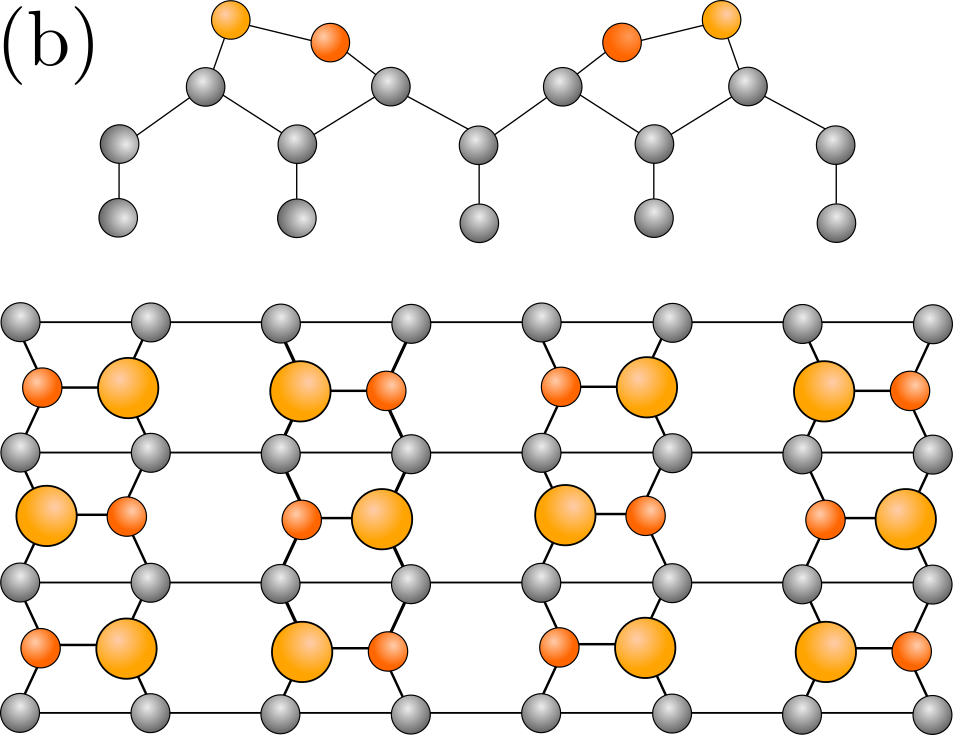
\includegraphics[width=0.8\textwidth]{graphics/c(4x2).png}
		\caption{The dimers are unstable to vertical buckling. The buckling pattern that was found to have the lowest surface energy is the c(4x2) reconstruction.}
		\label{c(4x2)}
		\end{subfigure}
		\caption{The structure of the silicon surface after forming dimer \textbf{(a)} and after buckling \textbf{(b)} is shown.}
		\label{Fig::dimer-configs}
	\end{figure}
\section{Phase Transition of the Si(0,0,1) Surface}
	The Si(001) surface exhibits an order-disorder phase transition from the disordered p(2x1) (\autoref{p(2x1)-symmetric}) phase to the ordered c(4x2) reconstruction at a critical temperature of about $T_c \approx 200~\text{K}$ \cite{tabata1987order}. This continuous phase transition will be of central importance in the following discussion. We say that the p(2x1) structure is disordered since the surface only appears during experiments to be in this phase due to thermal fluctuations and flipping of the dimers. \\
	
	The Silicon surface is strongly anisotropic which leads to long streaks of order along ($\parallel$) the dimer rows and short domains of order across ($\perp$) the dimer rows. In \cite{brand2023dimer} it was found that the ratio of correlation lengths is $\frac{\xi_{\parallel}}{\xi_{\perp}} \approx 5.2$. The lattice spacing along the dimer rows is $a_\parallel =	3.84~\text{\AA}$, while across it is $a_\perp =	2 a_\parallel =	7.68~\text{\AA}$ (see \autoref{Fig::SiliconDiamond}). \\
	
	To understand the phase transition of the Si(001) surface we need to have a general understanding of phase transitions.
\chapter{Phase Transitions}
	Under phase transitions in the most classical sense one understands the transition from an unordered state to an ordered state when changing an external parameter, mostly the temperature $T$, through a certain critical value, for example $T_c$. Phenomenologically one could say that the driving force behind the phase transition is the minimization of the free energy $F = U - TS $, with internal energy $U$ and entropy $S$. Below the critical temperature, the internal energy U is minimized which usually comes with some kind of ordering that depends on the microscopic hamiltonian.
	\newline
	\\
	\textbf{Mathematical definition:}
	
	In the \textbf{thermodynamic limit} (system volume $V \rightarrow \infty$ or number of sites $N \rightarrow \infty$), we can give a mathematical definition of a phase transition. Consider our system to be dependent on a set of coupling constants $[K]$, which for example can be temperature $T$, pressure $p$ or interaction strength $J$. We define the free energy per site as
	\begin{equation}
		f[K] =	\lim\limits_{N \rightarrow \infty} \frac{F[K]}{N}
	\end{equation}
	If the thermodynamic limit $\lim\limits_{N\rightarrow \infty}$ exists, we can give a precise definition of a phase boundary. The $d$ coupling constants $[K]$ span the so called phase diagram. The free energy density $f[K]$ is analytic almost everywhere in this $d$-dimensional phase space, except from the possibility of non-analyticities at certain points, lines, planes, etc. up to dimensionality $d-1$. The connected areas of analyticity are called \textbf{phases} and non-analyticitys with dimension $d-1$ are called \textbf{phase boundaries} or \textbf{critical manifolds}. Since $f[K]$ has to be continuous everywhere, the phase boundaries come in two classes:
	\begin{enumerate}
		\item at least one of the first derivatives $\frac{\partial f}{\partial K_i}$ is discontinuous across the phase transition. This case belongs to the \textbf{first-order phase transition}.
		\item all derivatives $\frac{\partial f}{\partial K_i}$ are continuous. This transition is called the \textbf{continuous phase transition}. 
	\end{enumerate}
	The free energy density gives reasonable, when the correlation length $\xi$, which is basically the spatial extent of fluctuations in the system, is much smaller than the system size L, so $\xi \ll L$. 
	The phase transition of the silicon surface belongs to the continuous phase transitions. 
	
	Phase transitions exhibit rich phenomena like the divergence of the correlation length $\xi$ at the critical point. The reason for the universality of this behavior across different systems will be outlined in the next section with the help of renormalization group theory.
	\section{Renormalization Group Considerations} \label{Section::RG}
	The renormalization group (RG) theory is a general framework to study phase transitions and particle physics. It uses scale invariance arguments, meaning the self-similarity properties of systems at different length scales, to systematically investigate properties of the system. In the following basic considerations as well as important results shall be presented. \\
	
	Imagine an infinite two dimensional lattice with ising-like spins on each site.  Just as Kadanoff \cite{kadanoff1966scaling} we consider a square of length $l$ in lattice spacing units $a=1$ and map  their combined $l^2$ spins to a single value $\pm l^2$. Afterwards we renormalize their combined block spin to be either $+1$ or $-1$. The new blocks of spins define a new ising like system, but on a different length scale with a new lattice spacing $la$ like shown in . The proposal is now that there exists a new set of coupling parameters $[K^l]$ so that the total free energy stays the same. In terms of the free energy density we can write 
	\begin{equation} \label{free-energy-density}
		f[K] =	l^{-2} f[K^l]~,
	\end{equation}
	\begin{figure}[htp]
		\centering
		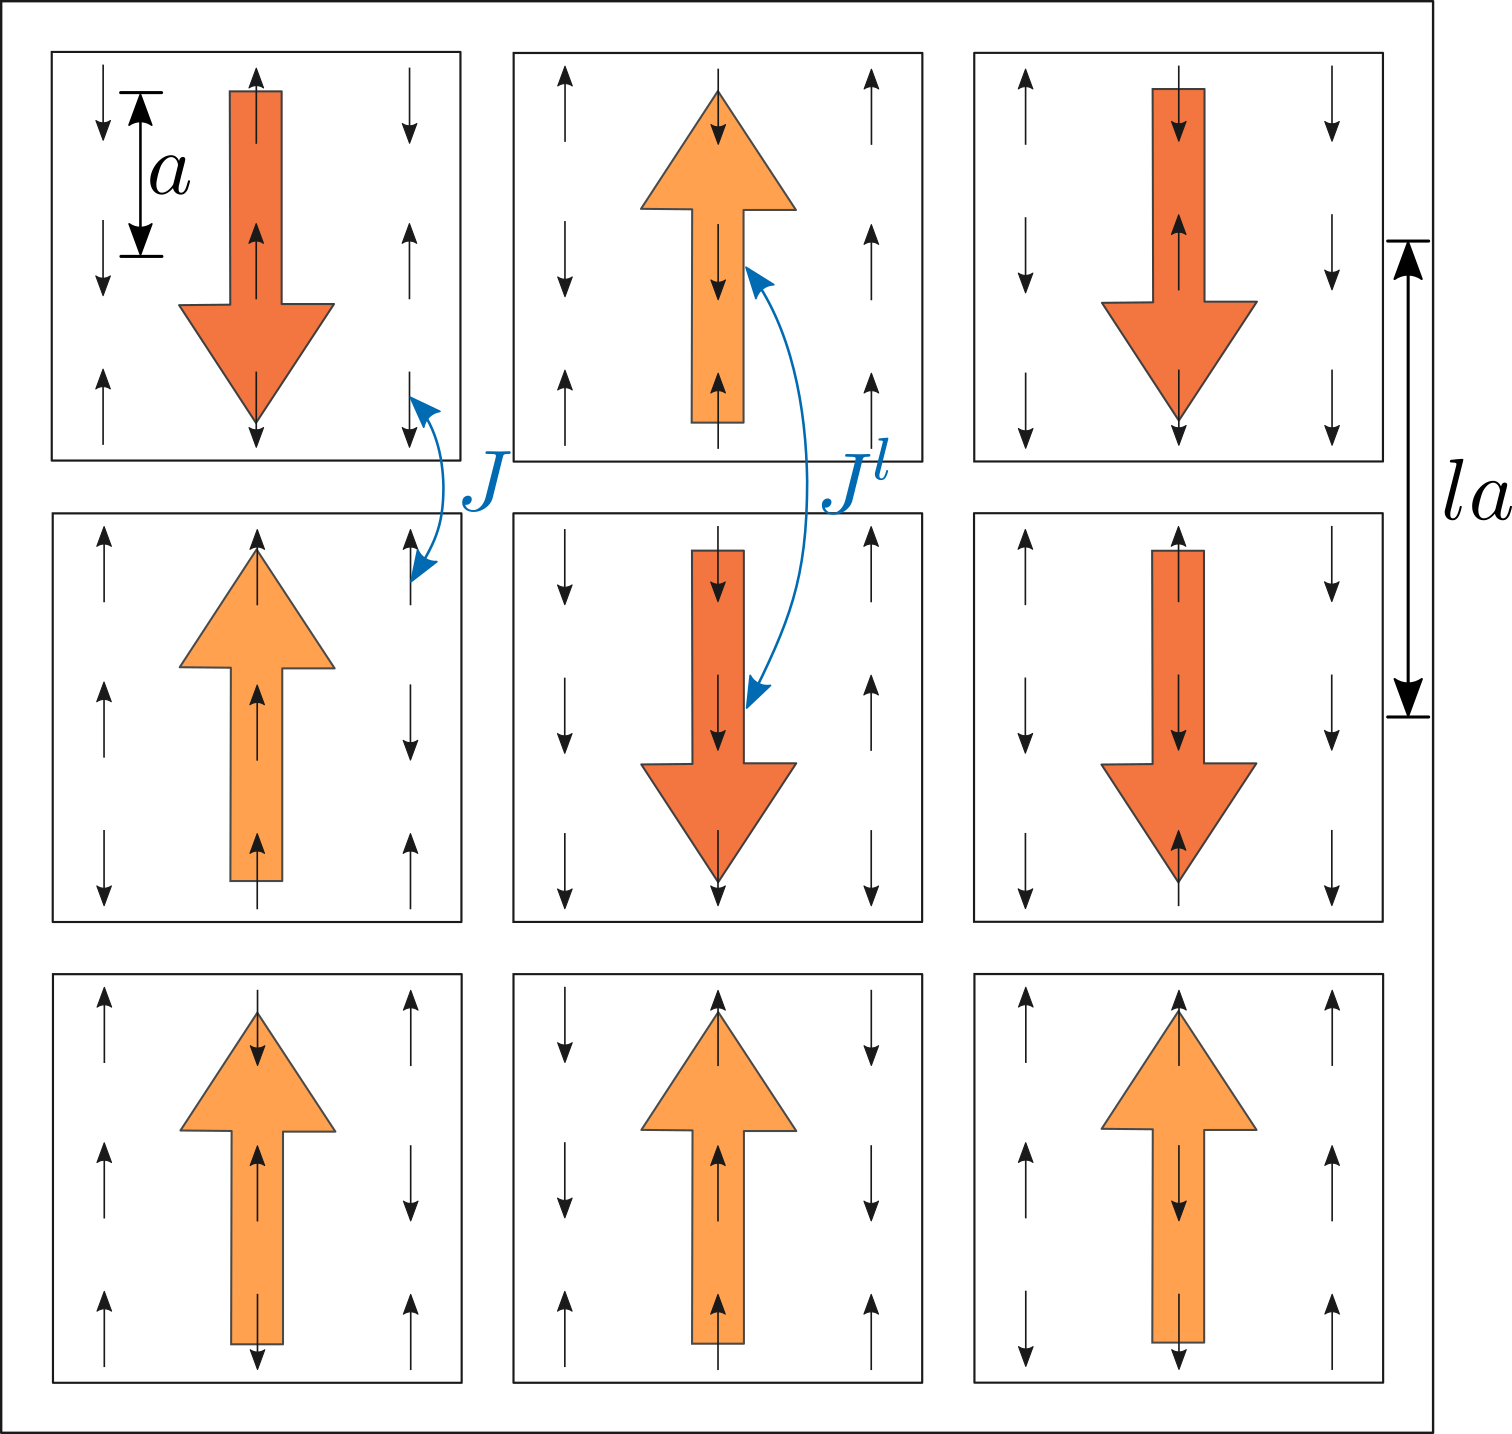
\includegraphics[width=0.7\linewidth]{graphics/RG-Iteration.png}
		\caption{In Kadanoffs block spin picture, one combines a number $l^2$ of spins to a new spin. The composite spin takes on the value of the majority of spins. The block spin is the standard example for a renormalization group transformation. Under the RG transformation, the relevant length scales change from $a$ to $la$.}
		\label{Fig::RG-Iteration}
	\end{figure}
	since the free energy density after the transformation has to be larger as we measure in a larger length scale. The same considerations can be made for the correlation length:
	\begin{equation}
		\xi[K] = l \xi[K^l]~.
	\end{equation}
	Suppose we know how the coupling constants change under an RG transformation $R_l$:
	\begin{equation}
		[K^l] =	R_l[K]~.
	\end{equation}
	This is the starting point for us to comprehend why phase transitions exhibit singular behavior. The idea is that even though the partition function is a sum of exponentials which are analytic in $[K]$, the singularities can arise after an infinite number of RG iterations. As we begin to apply RG transformations, our system traces out a trajectory in coupling constant space $\left([K^{(1)}] \rightarrow [K^{(2)}] \rightarrow [K^{(3)}] \rightarrow ...\right)$. This trajectory could in principle, for example, go in circles, but in practice, we almost always find that the system is attracted to fixed points. The behavior of a system near a fixed point is the origin of scaling and lets us extract important information, like the shape of the phase diagram.
	
	A fixed point of the RG	map satisfies
	\begin{equation}
		[K^{(*)}] =	R_l[K^{(*)}] ~.
	\end{equation}
	At this point the correlation length transforms according to
	\begin{equation}
		\xi[K^{(*)}] =	\xi[K^{(*)}] / l~,		
	\end{equation}
	meaning that the correlation length either has to be $0$ or $\infty$. The same is true for the free energy density. In proximity of a fixed point we may? write down the initial coupling constants as
	\begin{equation}
		K_i =	K_i^{(*)} + \delta K_i \qquad \text{and} \qquad K_i^l =	R_l(K_i^{(*)} + \delta K_i) =	K_i^{(*)} + \delta K_i^l~.
	\end{equation}
	A RG Transformation of those coupling constants is dependent on all coupling constants $K^l_i =	K^l_i[K] =	K^l_i(K_1^{(*)} + \delta K_1, K_2^{(*)} + \delta K_2, ...)$. We taylor expand $K_i^l$ around the fixed point $[K^{(*)}]$ to obtain the linearized RG Transformation:
	\begin{equation} \label{linearized-RG}
		K_i^l =	K_i^{(*)} + \sum_j \frac{\partial K_i^l}{\partial K_j} \bigg |_{K_j = K_j^{(*)}} \delta K_j + O((\delta K_j)^2) = K_i^{(*)} + \delta K_i^l + O((\delta K_j)^2) ~.
	\end{equation}
	We write down the partial derivatives as a matrix
	\begin{equation}
		M^l_{ij} =	\frac{\partial K_i^l}{\partial K_j} \bigg |_{K_j = K_j^{(*)}}
	\end{equation}
	and construct an eigenvalue problem:
	\begin{equation} \label{ev-problem}
		M^l k^{(\sigma)} =	\lambda^{(\sigma)}_l k^{(\sigma)}~,
	\end{equation}
	where $\sigma$ labels the eigenvalues. Because two consecutive RG Transformations by $l_1$ and $l_2$ have to yield the same result as one  with $l_1l_2$, we know that 
	\begin{equation}
		M^{l_1}M^{l_2} =	M^{l_1l_2}~, \qquad \text{implying that} \qquad \lambda_{l_1}^{(\sigma)} \lambda_{l_2}^{(\sigma)} =	\lambda_{l_1l_2}^{(\sigma)} ~.
	\end{equation}
	implying that
	\begin{equation}
		\lambda_{l_1}^{(\sigma)} \lambda_{l_2}^{(\sigma)} =	\lambda_{l_1l_2}^{(\sigma)} ~.
		\label{ev-equation}
	\end{equation}
	Setting $l_2 = 1$ yields $\lambda_{l_1}^{(\sigma)} \lambda_{1}^{(\sigma)} =	\lambda_{l_1}^{(\sigma)}$ which lets conclude that $\lambda_{1}^{(\sigma)} =	1$. Differentiating \autoref{ev-equation} with respect to $l_2$ yields
	\begin{equation}
			\begin{split}
			\frac{\text{d}}{\text{d}l_2} \left(\lambda_{l_1}^{(\sigma)} \lambda_{l_2}^{(\sigma)}\right) &= 	\frac{\text{d}}{\text{d}l_2} \lambda_{l_1l_2}^{(\sigma)} \\
			\lambda_{l_1}^{(\sigma)}  \left(\frac{\text{d}}{\text{d}l_2} \lambda_{l_2}^{(\sigma)}\right) +  			  \left( \frac{\text{d}}{\text{d}l_2} \lambda_{l_1}^{(\sigma)}\right) \lambda_{l_2}^{(\sigma)} &= l \frac{\text{d}}{\text{d}(l_1l_2)} \lambda_{l_1l_2}^{(\sigma)} \\
				\left(\frac{\text{d}}{\text{d}l_2} \lambda_{l_2}^{(\sigma)}\right) \lambda_{l_1}^{(\sigma)}   &= l \frac{\text{d}}{\text{d}(l_1l_2)} \lambda_{l_1l_2}^{(\sigma)}	~.
		\end{split}
	\end{equation}
	Setting now $l_2 =	1$ gives the differential equation
	\begin{equation}\label{RG-diff}
		\frac{\text{d}}{\text{d}l_2} \lambda_{l_2}^{(\sigma)} \bigg |_{l_2 =	1} \lambda_{l_1}^{(\sigma)}   \equiv y_\sigma \lambda_{l_1}^{(\sigma)} = l \frac{\text{d}}{\text{d}l_1} \lambda_{l_1}^{(\sigma)} \quad \Rightarrow \quad \frac{\text{d}}{\text{d}l_1} \lambda_{l_1}^{(\sigma)} =	\frac{y_\sigma}{l} \lambda_{l_1}^{(\sigma)} ~.		
	\end{equation}
	A solution to \autoref{RG-diff} is
	\begin{equation} \label{ev-form}
		\lambda_l^{(\sigma)} = l^{y_\sigma}	
	\end{equation}
	with $y_\sigma$ as defined above, being independent of $l$. This is an important result on the way to show the origin of scaling. Since the $k^{(\sigma)}$ are vectors in the coupling constant space, we deduce from \autoref{ev-problem} that some differences in coupling constants $\delta K$ grow or shrink when applying RG transformations, depending on the $\lambda_l^{\sigma}$. There are three cases:
	\begin{enumerate}
		\item \textbf{Relevant} directions and eigenvalues:	$|\lambda_l^{(\sigma)}| > 1$, meaning that $y_\sigma > 0$ and $\delta K$ in direction of $k^{(\sigma)}$ grow.
		\item \textbf{Irrelevant} directions and eigenvalues:	$|\lambda_l^{(\sigma)}| < 1$, meaning that $y_\sigma < 0$ and $\delta K$ in direction of $k^{(\sigma)}$ shrink.
		\item \textbf{Marginal} directions and eigenvalues:	$|\lambda_l^{(\sigma)}| = 1$, meaning that $y_\sigma = 0$ and $\delta K$ in direction of $k^{(\sigma)}$ do not change.
	\end{enumerate}
	After many RG transformations, only the relevant eigenvalues will be important, as the influence of the others will negligible in comparison. If we differ from the fixed point in a relevant direction, the differences to the fixed point will become larger and the RG transformation flow will flow out of the fixed point. Deviations in irrelevant direction will flow into the fixed point again. \\
	
	Consider a system with only one coupling constant, in this case the temperature, and choose $T$ in the vicinity of a fixed point $T^{(*)}$. Apply a RG transformation to $T$ so that $T^l =	R_l(T)$ and then consider the difference 
	\begin{equation} \label{temp-difference}
		T^l - T^{(*)} =	R_l(T) - T^{(*)}~. 
	\end{equation}
	Using \autoref{linearized-RG} we can rewrite
	\begin{equation}
		R_l(T) =	T^{(*)} + \delta T^l =	T^{(*)} + \frac{\partial T^l}{\partial T} \bigg |_{T =	T^{(*)}} \delta T =	T^{(*)} + \lambda_l \delta T
	\end{equation}
	since $M^l$ has only one component and $\delta T$ is therefore automatically in eigenvector direction. \autoref{temp-difference} then becomes in terms of the reduced temperature $ \varepsilon =	\frac{T - T^{(*)}}{T^{(*)}}$
	\begin{equation} \label{coupling-constant-ev-scaling}
		\varepsilon^{(l)} =	\lambda_l \varepsilon \overset{\text{\autoref{ev-form}}}{=} \varepsilon l^{y_\varepsilon}~.
	\end{equation}
	After $n$ RG iterations one obtains
	\begin{equation}
		\varepsilon^{(nl)} = \left( l^{y_\varepsilon}	\right)^n \varepsilon~.
	\end{equation}
	Now consider again how the correlation length transforms after $n$ RG transformations:
	\begin{equation} \label{xi-behavior}
		\xi(\varepsilon) =	l^n \xi(\varepsilon^{nl}) =	l^n \xi( l^{ny_\varepsilon} \varepsilon)
	\end{equation}
	Substituting $\tau =	l^{ny_\varepsilon} \varepsilon$ into \autoref{xi-behavior} yields
	\begin{equation} \label{RG-xi-scaling}
		\xi(\varepsilon) =	\tau^{1 / y_\varepsilon} \varepsilon^{-1/ y_\varepsilon} \xi(\tau)
	\end{equation}
	This is the origin of scaling and universality!
	\section{Universality and static scaling} \label{Section::Universality}
	The last section traced the origin of universality and scaling in phase transitions. This section will deal with the term universality and its implications in more detail. \\
	
	Scaling laws like \autoref{RG-xi-scaling} can be derived for many different quantities of a system. In the context of phase transitions, \textbf{static scaling} means the power law dependence of a system quantity \textbf{in equilibrium}, like the correlation length $\xi$, on a coupling parameter, like the temperature $T$. The exponent of this power law is called the \textbf{critical exponent}. Important scaling laws include the scaling of (in the notation of \cite{pelissetto2002critical})
	\begin{itemize}
		\item the specific heat $\boldsymbol{C_H}$: $T_c C_H \approx A^{\pm} |\varepsilon|^{-\alpha}$,
		\item the order parameter $\boldsymbol{\Psi}$ or $\boldsymbol{M}$: $|M| \approx B |\varepsilon|^{-\beta}$,
		\item the susceptibility $\boldsymbol{\chi}$: $\chi \approx C^{\pm} |\varepsilon|^{-\gamma}$,
		\item and the correlation length $\boldsymbol{\xi}$ : $\xi \approx f^{\pm} |\varepsilon|^{-\nu}$.		
	\end{itemize}
	The prefactors of the power laws are called the \textbf{critical amplitudes} and $\nu, \alpha, ...$ are the mentioned critical exponents. The superscript $\pm$ denotes whether the phase transition is approached from below $(-)$ or above $(+)$ the critical temperature $T_c$. The critical exponents are the same on both sides of the transition, but the amplitudes vary. \\
	
	These scaling laws are only valid in the thermodynamic limit for $\varepsilon \rightarrow 0$, so infinitely close to the critical point. Otherwise they exhibit \textbf{corrections to scaling} that result out irrelevant and marginal eigenvalues of the RG transformations as well as \textbf{finite size} corrections. \\
	
	Systems that share the same set of critical exponents belong to the same \textbf{universality class}. In the last section we motivated that this might be a result of symmetry considerations and indeed, it is found that which universality class a system belongs to usually only depends on
	\begin{itemize}
		\item the \textbf{symmetry group} of the system hamiltonian,
		\item the \textbf{dimensionality} of the problem,
		\item and whether the \textbf{interaction} between the components is \textbf{short-ranged}.
	\end{itemize}
	In contrast to the critical exponents, the critical amplitudes are not universal, but their ratios, for example $f^+/f^-$, are.\\
	
	The concept of universality is very useful to investigate real systems at the critical point. As a result of scale invariance and self similarity, the microscopic dynamics of a system become irrelevant at $\varepsilon =	0$ and its behavior can then be approximated by a simplified, hopefully exactly solvable model. \\
	
	The extraction of critical exponents is notoriously difficult for various reasons, one being the inaccessibility of the thermodynamic limit $\lim\limits_{N \rightarrow \infty}$, another \textbf{critical slowing down} (see \autoref{Section::Dynamic-Scaling}). The following section will explain the mentioned finite size corrections to static scaling and illustrate how one can make use of them to analyze critical exponents.
	\section{Finite size scaling and critical exponent extraction} \label{Section::FSS}
	Recall how the free energy density \autoref{free-energy-density} transforms and that it depends on the system size $L = l L^{(l)}	$:
	\begin{equation}\label{FSS-free-energy-scaling}
		f\left([K], L^{-1}\right) =	l^{-2} f\left([K^{(l)}], {L^{(l)}}^{-1}\right) = l^{-2} f\left([K^{(l)}], l{L}^{-1}\right)	 ~.
	\end{equation}
	Let $K_1 =	\varepsilon$ be the reduced temperature. Close to the critical point we can use \autoref{coupling-constant-ev-scaling} to write \autoref{FSS-free-energy-scaling} in terms of eigenvalues:
	\begin{equation}
				f\left(\varepsilon, K_2, ..., L^{-1}\right) = l^{-2} f\left(\varepsilon l^{y_\varepsilon}, K_2 l^{y_2}, ..., l{L}^{-1}\right)	 ~.
	\end{equation} 
	The system size behaves like a relevant eigenvalue with a value of
	\begin{equation}
		\lambda_L =	1 \qquad \text{implying that} \qquad y_L =	1 ~.
	\end{equation}
	This means that the system size has to be tuned to criticality to let the phase transition occur, which is in accord with our interpretation that phase transitions only occur in the thermodynamic limit, i.e. if $L^{-1} =	0$. As a result real, finite systems deviate from the behavior that the scaling laws dictate. For example, the actual correlation length cannot outgrow the system size $\xi \leq L$ and so the divergence of $\xi$ is rounded at the phase transition. Additionally the peak is shifted to a lower critical temperature \autoref{xi-divergence-FS}, so the phase transition appears to happen at a different point. \\
	\begin{figure}[htp]
		\centering
		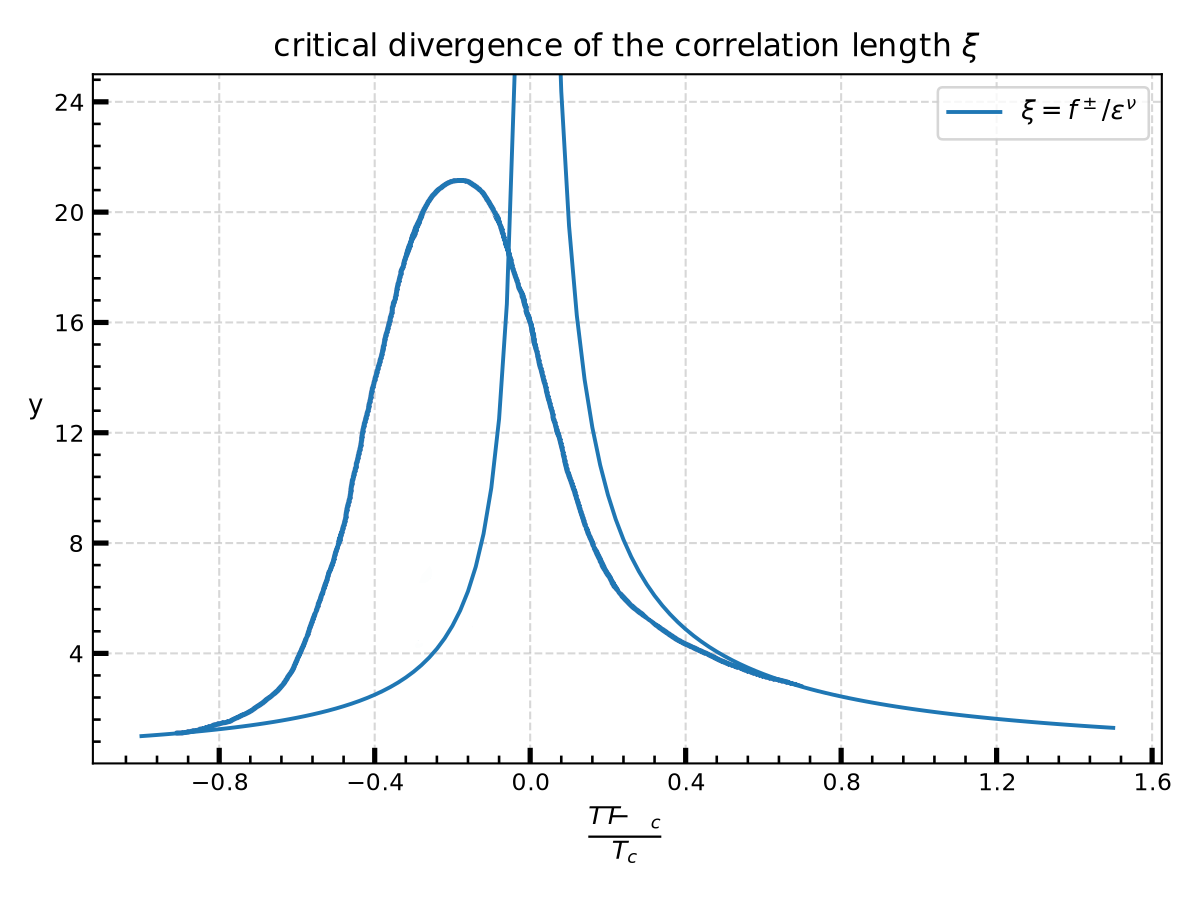
\includegraphics[width=0.7\linewidth]{graphics/xi-divergence-FS.png}
		\caption{PLACEHOLDER. In the thermodynamic limit, the correlation length $\xi$ diverges at the critical point according to a power law. For finite systems, the singularity of $\xi$ appears rounded and the peak position is shifted to a lower temperature.}
		\label{xi-divergence-FS}
	\end{figure} \\
	TODO: \\
	Consider again the correlation length and \autoref{xi-behavior}:
	\begin{equation}
		\xi(\varepsilon, L^{-1}) =	l \xi (\varepsilon l^{y_\varepsilon}, l L^{-1}) = \varepsilon^{-\nu} F_\xi (L^{-1} \varepsilon^{-\nu})
 	\end{equation} 
 	with $F_\xi$ as in \autoref{RG-xi-scaling}. Introducing a new scaling function $F' =	(L \varepsilon^\nu)^{-1} F_\xi$ yields
 	\begin{equation}
 		\xi(\varepsilon, L^{-1}) = \varepsilon^{-\nu} (L\varepsilon^\nu) F' (L \varepsilon^{\nu}) =	L	F'(L \varepsilon^\nu)~.	
 	\end{equation}
 	In the limit $L \rightarrow \infty$ and close to $\varepsilon =	0$, $\xi$ has to scale like $\xi(\varepsilon, 0) \propto \varepsilon^{-\nu}$. Taylor expansion around $\varepsilon =	0$ somehow yields \cite{goldenfeld2018lectures}
 	\begin{equation} \label{Eq::FSS-Scaling-L/xi}
 		\frac{L}{\xi(\varepsilon, L^{-1})} =	A + B \varepsilon L^{1/\nu} + O(\varepsilon^2)
 	\end{equation}
 	TODO end \\
 	
 	This equation is an important result since it can be used to calculate two important quantities. Firstly, curves of $L/\xi(\varepsilon, L^{-1})$ for different $L$ intersect at the critical point $\varepsilon = 0$, so by determining this intersection one can extract the critical temperature $T_c$, which is usually not known a priori. Secondly by computing the gradient
 	\begin{equation}
 		\frac{\partial}{\partial \varepsilon} \left(\frac{L}{\xi(\varepsilon, L^{-1})}\right) =	B L^{1/\nu}
 	\end{equation}
 	for various $L$, one can determine the critical exponent $\nu$. This method is easier than, for example, trying to fit to the original scaling law \autoref{RG-xi-scaling} because of the reasons mentioned at the end of \autoref{Section::Universality}. There are numerous quantities that behave like \autoref{Eq::FSS-Scaling-L/xi}. They are called phenomenological couplings $R$  and they can be shown \cite{hasenbusch2008critical} to follow
 		\begin{equation}
 		R(\varepsilon, L) =	R^* + r' \varepsilon L^{y_\varepsilon} + ... + c_\omega L^{-\omega}~. 
 	\end{equation}
 	\subsection{Binder Cumulant} \label{Sec::Binder-Cumulant}
 	A popular quantity to apply \autoref{Equation::FSS-Scaling-L/xi} (TODO	unclear) is the Binder cumulant $U_L$, introduced by K. Binder in \cite{binder1981finite}. It is defined as
 	\begin{equation} \label{Eq::Def-Binder-Cum}
 		U_L =	\frac{\langle M_L^4 \rangle}{\langle M_L^2 \rangle^2}~,
 	\end{equation}
 	$M_L$ being the order parameter of a system of size $L$. $\left\langle~\cdot~\right \rangle$ denotes the ensemble average, meaning the average over different realizations of the same system. It's finite size scaling is given in analogue to \autoref{Equation::FSS-Scaling-L/xi} by
 	\begin{equation}
 		U_L =	U_L^* + U \varepsilon L^{1/\nu} \left(1 + W L^{-\omega} + ...\right)~,
 	\end{equation}
 	including the corrections resulting out of the largest irrelevant eigenvalue $1/|y_1| =	\omega $.
 	In practice, to extract the critical exponent $\nu$, one fits to
 	\begin{equation} \label{Eq::FSS-dU_dT}
 		\ln \left(\frac{\partial U_L}{\partial \varepsilon}\right) \approx	\ln \left(U L^{1/\nu} \right) =	\ln (U) + \frac{1}{\nu} \ln (L) ~.
 	\end{equation}
  	$U_L$ has a value of $U_L = 1$ far below the phase transition, approaches $U_L =	3$ above the phase transition and exhibits the intersection in between at $U_L =	U_L^*$. It is generally easy to compute and extract out of the system.
  	
  	\subsection{The correlation length ratio $\frac{\xi}{L}$}
  	TODO
  	
	\section{Dynamic Scaling and the Kibble-Zurek mechanism} \label{Section::Dynamic-Scaling}
	\subsection{The relaxation time $\tau$ and the critical exponent $z$}
	With the Binder cumulant we saw a way to extract the static scaling exponent $\nu$. Aside static scaling, phase transitions show another phenomenon, called \textbf{dynamic scaling}. The topic of dynamic critical phenomena deals with how long the fluctuations in the system on the largest lengthscale take to equilibrate. This time is called the the \textbf{relaxation time} and it is found to scale like
	\begin{equation}
		\tau =	\tau_\xi \xi(\varepsilon)^z~,
	\end{equation}
	with the new \textbf{dynamic critical exponent} z. (TODO RG explanation for this scaling?). \\
	
	Plugging in the known scaling of $\xi(\varepsilon)$ from \autoref{Section::Universality} yields
	\begin{equation}
		\tau = \tau_\xi \xi(\varepsilon)^z =\tau_\xi	\left(f^{\pm} |\varepsilon|^{-\nu}\right)^z :=	\tau_\varepsilon |\varepsilon|^{-\nu z} ~.
	\end{equation}
	As the correlation length diverges, so does the relaxation time. This makes intuitively sense, since infinite correlation length implies that infinitely far apart components of the system had ''time to talk'', and for that to happen, it would take an infinite amount of time. This is what is meant with the in \autoref{Section::Universality} mentioned critical slowing down. As a system approaches $\varepsilon \rightarrow 0$, it takes longer and longer to equilibrate. It then becomes computationally a challenge to let large systems equilibrate. But since static scaling laws involve only quantities in equilibrium and are only valid in the thermodynamic limit for $\varepsilon \rightarrow 0$, large, critical systems have to be considered.  This dilemma was partially solved by the finite size techniques of \autoref{Section::FSS}.
	\subsection{Quenches and the freezeout of domains}
	The \textbf{Kibble-Zurek mechanism} (KZM) \cite{zurek1985cosmological, zurek1996cosmological} shall be a central point of the upcoming investigations and will be explained in the following. \\
	
	Consider a linear quench, meaning the cooling down of a system linear in time $t$(?). We characterize the speed of cooling by the \textbf{quench timescale} $\tau_Q$:
	\begin{equation} \label{Eq::Linear-Quench}
		\varepsilon(t) =	\frac{t}{\tau_Q}~.
	\end{equation}
	For slow quenches sufficiently far away from the critical point, the system will evolve adiabatically, meaning that system quantities like $\xi$ assume their equilibrium values. As we get closer to the phase transition, the change in $\xi$ becomes faster and faster since it's time derivative $\frac{\partial}{\partial t} \xi(\varepsilon(t))$ diverges. At the latest when $\frac{\partial}{\partial t} \xi(\varepsilon(t))$ outgrows the speed of sound the system cannot keep up with the change in the equilibrium correlation length and therefore diverges from it's equilibrium behavior \autoref{Fig::Freezeout}. The timepoint $\hat{t}$ of divergence from the equilibrium behavior is called the \textbf{freezeout} since the current state of the system effectively becomes frozen in comparison with the equilibrium values. One Assumption of the KZM is that this freezeout roughly happens when the current relaxation time $\tau$ equals the time that is left until the critical point is crossed:
	\begin{equation}
		\tau(\hat{t}) = \hat{t}~.
	\end{equation}
	\begin{figure}[htp] 		
		\centering
		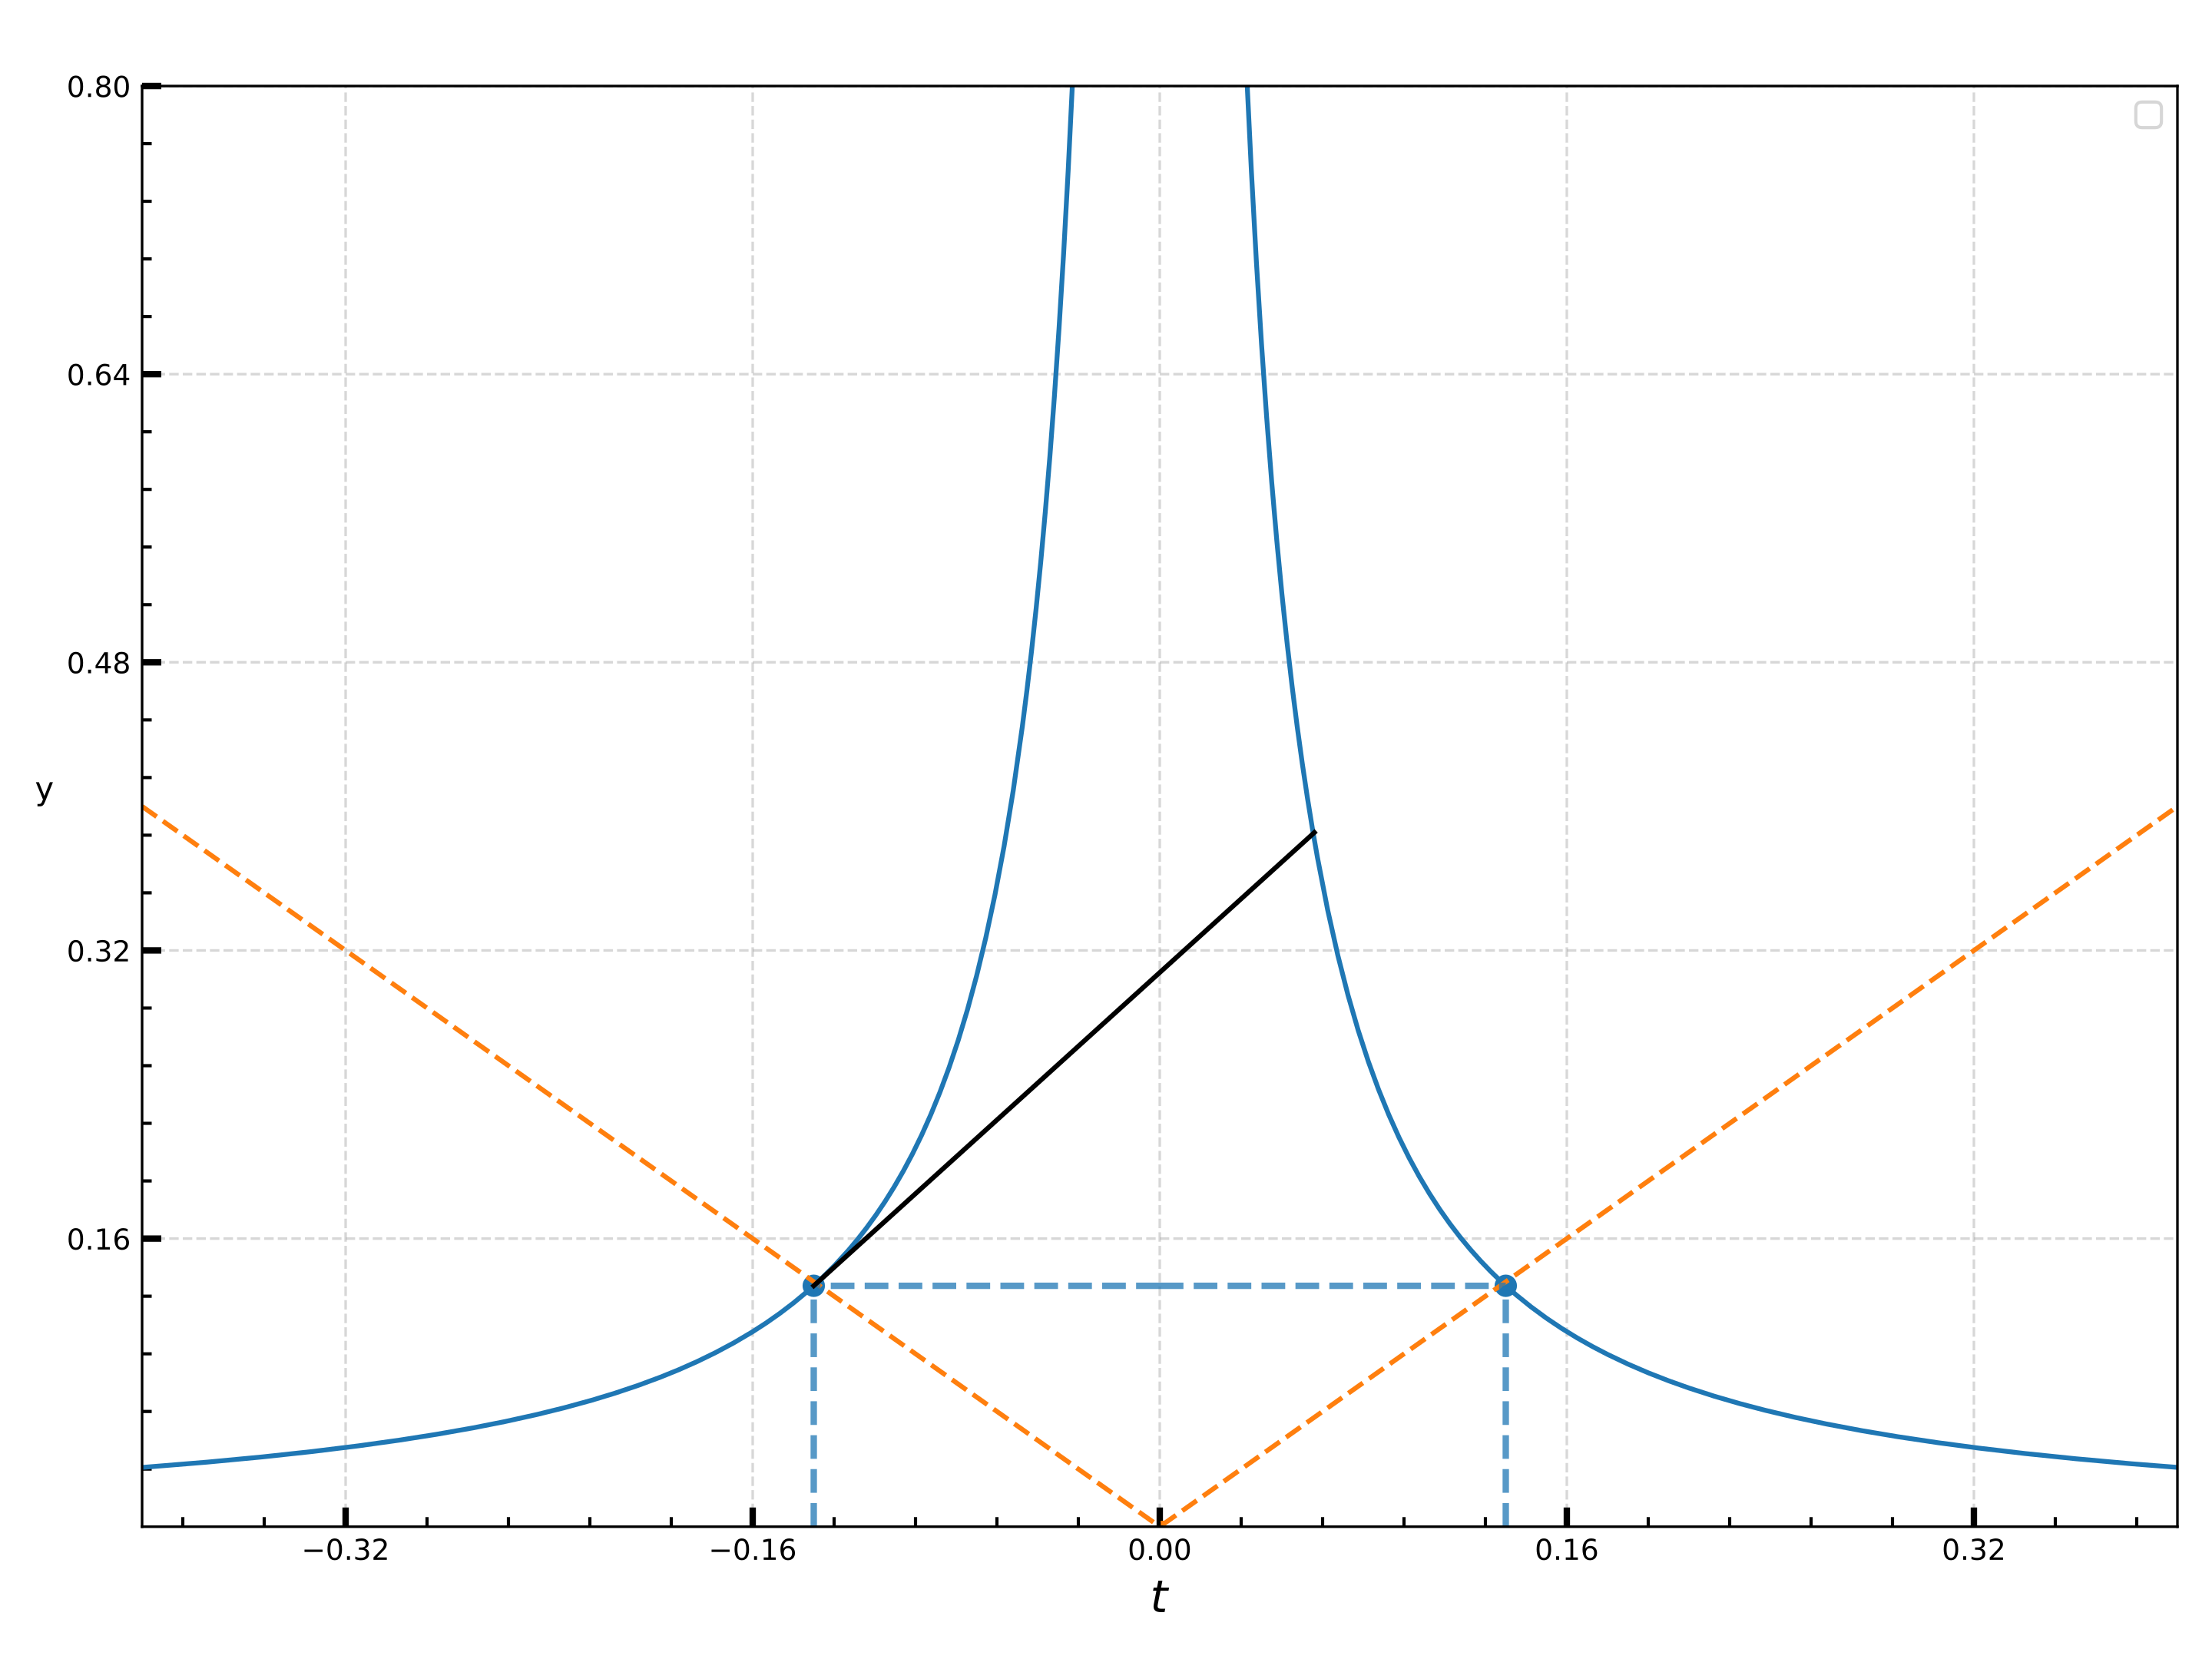
\includegraphics[width=0.7\linewidth]{graphics/xi-divergence-symmetric.png}
		\caption{PLACEHOLDER. The freezeout of the current state of the system happens roughly at $\tau(\hat{t}) =	\hat{t}$. After that, the system continues to evolve in its maximum speed until the critical point is crossed and the actual values intersect with the equilibrium values.}
		\label{Fig::Freezeout}
	\end{figure}
	Another is that the system quantities after the quench will have only reached approximately their equilibrium value at $\hat{t}$. Combining
	\begin{equation}
		\hat{t} =	\varepsilon(\hat{t}) \tau_Q \qquad \text{and} \qquad  \hat{t} =	\tau(\hat{t}) = \tau(\varepsilon(\hat{t})) =	\tau_\varepsilon \big | \varepsilon(\hat{t}) \big |^{-\nu z}
	\end{equation} 
	yields the reduced temperature at $\hat{t}$:
	\begin{equation}
		\big|\varepsilon (\hat{t}) \big| =	\left(\frac{\tau_\varepsilon}{\tau_Q} \right)^{\frac{1}{1 + \nu z}} ~.
	\end{equation}
For $\xi$ this means:
	\begin{equation} \label{Eq::KZM-scaling}
		\xi \approx \hat{\xi} := \xi(\varepsilon(\hat{t})) =	\xi_0 / |\varepsilon(\hat{t})|^{\nu} =	\xi_0 \bigg| \frac{\tau_Q}{\tau_\varepsilon} \bigg |^{\frac{\nu}{1 + \nu z}} ~,
	\end{equation}
	so the frozen value of the correlation length scales with the quench timescale like $\hat{\xi} \propto \tau_Q^{\frac{\nu}{1 + \nu z}}$~.
	The freezeout of the correlation length implies domains of order $\propto \hat{\xi}^2$. The domains of order are separated by \textbf{domain walls}, which represent a defect in the order of the surface. Such defects may have influences on different properties of the surface, including conductivity, an important value for the semi conductor industry. Knowledge of how the defect density on the surface behaves might help to prepare ideal silicon surfaces.  
	\chapter{Simulating Dynamics}
	While most numerical studies of phase transitions rely on monte carlo techniques, this work, inspired by Laguana and Zurek \cite{laguna1997density}, focuses on the use of \textbf{stochastic differential equations}. Their mathematical basics and a derivation of a Langevin equation for our case  will be outlined in the following.
	\section{Stochastic differential equations and the Langevin equation}
		Put simply, stochastic differential equations are the stochastic generalizations of common differential equations like
		\begin{equation} \label{Eq::diff-eq}
			y(t + dt) =	y(t) + A(y(t), t) dt ~.
		\end{equation}
		\autoref{Eq::diff-eq} describes a \textbf{continuous, memoryless, deterministic} process. For every timepoint $t + dt$ one can predict the value $y(t+dt)$ knowing the values $y(t), dt $ and $t$. SDEs describe continuous, memoryless \textbf{stochastic} processes, also called continuous \textbf{markov processes}, meaning for every timepoint we can assign definite probabilities to all possible $y(t + dt)$. These properties impose relatively strict limitations on a generalization of \autoref{Eq::diff-eq}. It turns out, that the generalization must be of the form \cite{gillespie1996mathematics}.
		\begin{equation} \label{Eq::std-langevin-eq}
			y(t + dt) =	y(t) + A(y(t), t) dt + D^{1/2} \left(y(t), t\right) n(t) (dt)^{1/2}~.
		\end{equation}
	 	$n(t)$ is a sample value of a normal distribution around zero with standard deviation one $\mathcal{N}(0,1)$. \autoref{Eq::std-langevin-eq} is called the standard form \textbf{Langevin equation} and it represents an update formula for the continuous markov process. To obtain the widely used \textbf{differential }or \textbf{white noise }form of the Langevin equation, we define the \textbf{Gaussian white noise process} $\Gamma(t)$ by
	 	\begin{equation}
	 		\Gamma(t) :=	\lim\limits_{dt \rightarrow 0} \mathcal{N}(0, 1/dt) \equiv \frac{n(t)}{(dt)^{1/2}},
	 	\end{equation}
 		rearrange \autoref{Eq::std-langevin-eq}
 		\begin{equation}
 			\frac{y(t + dt) - y(t)}{dt} =	A(y(t), t) + D^{1/2} (y(t), t) \frac{n(t)}{(dt)^{1/2}}
 		\end{equation}
 		and take the limit $dt \rightarrow 0$, leading to
 		\begin{equation} \label{Eq::Differential-Langevin-eq}
 			\frac{d}{dt} y(t) =	A(y(t), t) + D^{1/2}(y(t), t) \Gamma(t)~.
 		\end{equation}
 		$A(y(t), t)$ is called the \textbf{drift} and $D(y(t), t)$ is called the \textbf{diffusion} function. Important properties of the white noise process $\Gamma(t)$ are
 		\begin{equation}
 			\left \langle \Gamma(t) \right \rangle = 0 \qquad \text{and} \qquad  			\left \langle \Gamma(t) \Gamma(t + t')\right \rangle =	\delta(t') ~.
 		\end{equation} 
 		
 		\subsection{Ornstein-Uhlenbeck process and Brownian motion} \label{Section::Brownian-Motion}
 		The Ornstein-Uhlenbeck process is central to the mathematical description of Brownian motion, which will be used to model the movement of the silicon dimers. The Ornstein-Uhlenbeck process is a continuous Markov process with drift and diffusion functions of the form
 		\begin{equation}
 			A(y(t), t) =	- \frac{1}{\tau} y(t) \qquad \text{and} \qquad D(y(t), t) =	c~.
 		\end{equation}
 		The constants $\tau$ and $c$ are the \textbf{relaxation time} and the \textbf{diffusion constant}. Plugging the drift and diffusion functions into \autoref{Eq::std-langevin-eq} yields
 		\begin{equation}\label{Eq::OU-Langevin}
 			 			y(t + dt) =	y(t) - \frac{1}{\tau} y(t) dt + c^{1/2} n(t) (dt)^{1/2}~.
 		\end{equation}
 		$y(t)$ is normally distributed, since $y(dt)$ is normally distributed as the sum of a constant depending on $y(0)$ and the normal variable $n(dt)$. $y(2dt)$ is normally distributed being the linear combination of two statistically independent normal variables $y(dt)$ and $n(2dt)$. Continuation shows the normal distribution of $y(t)$.
 		The differential equations for the first and second moment of $y$ are
 		\begin{align}
 			&\left \langle y(t + dt) \right \rangle =	\left \langle y(t) \right \rangle - \frac{1}{\tau} \left \langle y(t) \right \rangle dt \qquad \qquad \qquad \qquad  \text{and} \\
 			&\left \langle y^2(t + dt) \right \rangle =	\left \langle y^2(t) \right \rangle - \frac{2}{\tau} \left \langle y^2(t) \right \rangle dt  + c dt
 		\end{align}
 		Solving these equations with the initial condition $y(0) =	y_0$ yields the mean
 		\begin{equation}
 			\left \langle y(t) \right \rangle =	 y_0 e^{-t/\tau}
 		\end{equation}
 		and the variance 
 		\begin{equation}
 			\left \langle y^2(t) \right \rangle - \left \langle y(t) \right \rangle^2 =	\frac{c\tau}{2} \left(1 - e^{-2t /	\tau)}\right)~.
 		\end{equation}
 		of $y(t)$. This determines the distribution of $y(t)$ to be
 		\begin{equation} \label{Eq::OU-Distribution}
 			y(t) =	\mathcal{N}\left(y_0 e^{-t/\tau}, \frac{c\tau}{2} \left(1 - e^{-2t /	\tau)}\right)\right) \overset{t \rightarrow \infty}{=} \mathcal{N}\left(0 , \frac{c\tau}{2}\right) ~.
 		\end{equation}
 		Consider now a particle that is coupled to a reservoir of temperature $T$ resulting in a dissipative drag force $- \frac{\eta}{m} p(t)$ proportional to a dampening constant $\eta$ as well as a fluctuating force $F(T)$. By Newton's second law, its equation of motion is given by
 		\begin{equation}
 			\frac{\text{d}}{\text{dt}} p(t) =	- \frac{\eta}{m} p(t) + m F(t)~,
 		\end{equation}
 		which we identify with the Langevin equation for the Ornstein-Uhlenbeck process \autoref{Eq::OU-Langevin}
 		\begin{equation}
 			\frac{\text{d}}{\text{dt}} p(t) =	- \frac{1}{\tau} p(t) + { c^{1/2}}{m} \Gamma(t).
 		\end{equation}
 		From classical statistical thermodynamics we know that the velocity of the particle will eventually be distributed in a Maxwell-Boltzmann fashion:
 		\begin{equation} \label{Eq::Maxwell-Boltzmann}
 			p(t\rightarrow \infty) =	\mathcal{N}(0, m k_B T)~.
 		\end{equation}
 		Comparing \autoref{Eq::OU-Distribution} and \autoref{Eq::Maxwell-Boltzmann} shows that
 		\begin{equation}
 			\frac{c \tau m}{2} =	k_B T \qquad \quad \text{or equivalently} \qquad \quad c =	\frac{2 k_B T \eta }{m^2}~, 			
 		\end{equation}
 		implying that the dampening constant or respectively the relaxation time and the diffusion constant are not independent. For a particle in a potential $V(x)$ one eventually obtains the equations of motions
 		\begin{align} \label{Eq::Langevin-eq-motion-set-x}
 			&\frac{\text{d}}{\text{dt}} x(t) =	\frac{1}{m} p(t) \qquad \text{and}\\
 			\label{Eq::Langevin-eq-motion-set-p}
 			&\frac{\text{d}}{\text{dt}} p(t) =	- \frac{\eta}{m} p(t) - \frac{\partial V(x)}{\partial x} + \sqrt{2 k_B T \eta } \Gamma(t) ~.
 		\end{align} 	
 		Methods of solution of the Langevin equation will be presented in \autoref{Section::Numerical-methods}. But first we will talk about the applicability of the Langevin equation for the silicon surface.
	\section{Caldeira-Leggett Master equation}
		\subsection{Motivation of the master equation}
		The silicon surface is a complex system subject to quantum mechanical interactions in between the surface atoms, as well as the silicon bulk and it is therefore anything but clear that we can use a classical Langevin equations to approximate its behavior.\\
		
		A quantum mechanical microscopic theory is needed to live up to the silicon surface. Systems that are coupled to an environment are subject of the theory of open quantum systems, which will be used to derive a set of coupled Langevin equations. \\
		
		Consider the \textbf{Caldeira-Leggett model} \cite{caldeira1981influence} for a quantum mechanical particle of mass $m$, moving in a potential $V(\hat{x})$. We can write down it's \textbf{free Hamiltonian} $\hat{H}_S$ as 
		\begin{equation}
			\hat{H}_S =	\frac{1}{2m} \hat{p}^2 + V(\hat{x})~,
		\end{equation}   
		with the position and momentum operators $\hat{x}$ and $\hat{p}$. The bath, which is the silicon bulk, is modeled as a set of harmonic oscillators with frequencies $\omega_n$. The bath hamiltonian can be written in terms of the bosonic annihilation and creation operators $\hat{b}_n^\dagger$ and $\hat{b}_n$, or in terms of the canononically conjugated position $\hat{x}_n$ and momentum $\hat{p}_n$ operators of the $n$-th oscillator:
		\begin{equation}
			\hat{H}_B =	\sum_n \hbar \omega_n \left(\hat{b}_n^\dagger \hat{b}_n + \frac{1}{2} \right) =	\sum_n \left(\frac{1}{2 m_n} \hat{p}_n^2 + \frac{1}{2} m_n \omega_n^2 \hat{x}_n^2 \right)
		\end{equation}
		We assume that the coordinate $\hat{x}$ of the Brownian particle is linearly coupled to th coordinates $\hat{x}_n$ of the bath oscillators, yielding for the interaction Hamiltonian $\hat{H}_I$
		\begin{equation}
			\hat{H}_I =	- \hat{x} \otimes \sum_n \kappa_n \hat{x}_n =	-\hat{x} \otimes \sum_n \kappa_n \sqrt{\frac{\hbar}{2 m_n \omega_n}} \left(\hat{b}_n + \hat{b}_n^\dagger\right) =	- \hat{x} \otimes \hat{B} ~,
		\end{equation}
		with the coupling constants $\kappa_n$. To ensure positivity of the combined Hamiltonian $\hat{H}_{SB}$, a \textbf{counter-term}
		\begin{equation}
			\hat{H}_c =	\sum_n \frac{\kappa_n^2}{2 m_n \omega_n^2} \hat{x}^2 
		\end{equation}
		is added. The counter term is in the following absorbed into the system hamiltonian. The hamiltonian of the combined system, or the universe, is given by
		\begin{equation}
			\hat{H}_{SB} = \hat{H}_S + \hat{H}_B + \hat{H}_I~.
		\end{equation}
		Since it is neither possible, nor required to solve the dynamics of the whole hamiltonian, we will be looking for a probabilistic description of the surface. In the quantum mechanical terms this means we will derive an equation for the system  density matrix $\hat{\rho}_{S}$. Starting point is the von Neumann equation for $\boldsymbol{\hat{\rho}}_{SB} :=	e^{i \left(\hat{H}_S + \hat{H}_B\right)t} \hat{\rho}_{SB} e^{-i \left(\hat{H}_S + \hat{H}_B\right)t}$ in \textbf{interaction picture} with respect to $\hat{H}_S + \hat{H}_B$:
		\begin{equation} \label{Eq::OQS-Startpoint}
			\frac{\partial}{\partial t}\boldsymbol{\hat{\rho}}_{SB}(t) =	- i \left[\boldsymbol{\hat{H}}_I(t), \boldsymbol{\hat{\rho}}_{SB}(t) \right] ~.
		\end{equation}
		To derive an equation for $\boldsymbol{\hat{\rho}}_S$ the reservoir degrees of freedom are traced out:
		\begin{equation} \label{Eq::Tracing-Out-Reservoir}
			\begin{split}
							\frac{\partial}{\partial t} \boldsymbol{\hat{\rho}}_S(t) &=	\text{tr}_B \left \lbrace \frac{\partial}{\partial t} \boldsymbol{\hat{\rho}}_{SB}(t) \right \rbrace =	-i~\text{tr}_B \left\lbrace \left[\boldsymbol{\hat{H}}_I(t), \boldsymbol{\hat{\rho}}_{SB}(t)\right] \right\rbrace  \\
							&=	-i~\text{tr}_B \left\lbrace \left[\boldsymbol{\hat{H}}_I(t), \boldsymbol{\hat{\rho}}_{SB}(0)\right] \right \rbrace - \int_{0}^{t} dt'~ \text{tr}_B \left\{  \left[\boldsymbol{\hat{H}}_I(t), \left[\boldsymbol{\hat{H}}_I(t'), \boldsymbol{\hat{\rho}}_{SB}(t') \right]\right]  \right\} \\
							&=- \int_{0}^{t} dt'~ \text{tr}_B \left\{  \left[\boldsymbol{\hat{H}}_I(t), \left[\boldsymbol{\hat{H}}_I(t'), \boldsymbol{\hat{\rho}}_S(t') \otimes \overline{\rho}_B \right]\right]  \right\}
			\end{split}
		\end{equation}
		The second line in \autoref{Eq::Tracing-Out-Reservoir} is obtained by integrating \autoref{Eq::OQS-Startpoint} and solving for $\boldsymbol{\hat{\rho}}_{SB}(0)$. Under the \textbf{Born approximation}, which assumes that the reservoir density matrix is stationary and we can decompose $\boldsymbol{\hat{\rho}}_{SB}(t) = \boldsymbol{\hat{\rho}}_S(t) \otimes \overline{\rho}_B$, the trace $\text{tr}_B \left\lbrace \left[\boldsymbol{\hat{H}}_I(t), \boldsymbol{\hat{\rho}}_{SB}(0)\right] \right \rbrace =	0$ vanishes, yielding the third line of \autoref{Eq::Tracing-Out-Reservoir}. Afterwards we apply the \textbf{markov approximation} \cite{landi2022nonequilibrium} by first replacing $\boldsymbol{\hat{\rho}}_S(t') \rightarrow \boldsymbol{\hat{\rho}}_S(t)$, then substituting $\tau =t - t'$, as well as sending the upper limit of the integral to infinity. This is permissible as the integrand disappears sufficiently fast. We obtain the \textbf{Redfield-II} master equation
		\begin{equation} \label{Eq::Redfield-II}
			\frac{\partial}{\partial t} \boldsymbol{\hat{\rho}}_S(t) = - \int_{0}^{\infty} d\tau~ \text{tr}_B \left\{  \left[\boldsymbol{\hat{H}}_I(t), \left[\boldsymbol{\hat{H}}_I(t - \tau), \boldsymbol{\hat{\rho}}_S(t) \otimes \overline{\rho}_B \right]\right]  \right\} ~.
		\end{equation}
		Transforming \autoref{Eq::Redfield-II} back to the Schrödinger picture gives
		\begin{equation} \label{Eq::Caldeira-Legget-Startpoint}
			\frac{\partial}{\partial t} {\hat{\rho}}_S(t) =	-i~\left[\hat{H}_S, \rho_S(t)\right] - \int_{0}^{\infty} d\tau~ \text{tr}_B \left\{  \left[{\hat{H}}_I, \left[{\boldsymbol{\hat{H}}}_I(- \tau), {\hat{\rho}}_S(t) \otimes \overline{\rho}_B \right]\right]  \right\}~.
		\end{equation}
		The integral in the second term of \autoref{Eq::Caldeira-Legget-Startpoint} can be rearranged (\autoref{Section::Appendix-Caldeira-Legget}) to 
		\begin{equation} \label{Eq::CD-Trace-with-Kernels}
			\int_{0}^{\infty} d\tau \left(\frac{i}{2} D(\tau) \left[\hat{x}, \left\{\boldsymbol{\hat{x}}(-\tau). \hat{\rho}_S(t)\right\}\right] - \frac{1}{2} D_1(\tau) \left[\hat{x}, \left[\boldsymbol{\hat{x}}(-\tau) , \hat{\rho}_S(t)\right]\right]\right)~,
		\end{equation}
		with the noise kernel $D_1(\tau)$ and dissipation kernel $D(\tau)$ defined as in \autoref{Section::Appendix-Caldeira-Legget}. In the markov approximation we already mentioned that the integrand decays sufficiently fast. This is because the noise and dissipation kernels disappear on the timescale of the relaxation $\tau_B$ of the reservoir. When doing the markov approximation we assume that this timescale is much shorter than the relaxation time of the system $\tau_S$. We now make use of this again by approximating $\boldsymbol{\hat{x}}(-\tau)$ in the integrand by its free dynamics
		\begin{equation}
			\boldsymbol{\hat{x}}(-\tau) =	\hat{x} - \hat{p} \tau~.
		\end{equation}
		Plugging this approximation into \autoref{Eq::CD-Trace-with-Kernels} enables to evaluate the integrals (see \autoref{Section::Appendix-Caldeira-Legget}). This eventually results in the \textbf{Caldeira-Leggett master equation}
		\begin{equation} \label{Eq::Caldeira-Leggett-Master-equation}
			\frac{\text{d}}{\text{dt}} \rho_S(t) =	\underbrace{-i\left[\hat{H}_S, \rho_S(t) \right]}_{\text{free dynamics}} - \underbrace{i \gamma \Big [\hat{x}, \big\{\hat{p}, \rho_S(t)\big\}\Big ]}_\text{dissipative term} - \underbrace{2 \eta m k_B T \Big [\hat{x}, \big[\hat{x}, \rho_S(t)\big]\Big ]}_\text{thermal fluctuations}~.
		\end{equation}
	$\gamma$ is a damping constant that enters the calculation through a parametrization of the spectral density function. The first term in the Caldeira-Leggett master equation describes the free dynamics of the system and resembles the form of the \textbf{von Neumann} equation. The second term is the dissipative part proportional to the damping constant $\eta$, which enters the calculation through the parameterization of the spectral density function \autoref{???}. The thermal fluctuations of the reservoir are captured in the third term proportional to the temperature $T$ determined by the state of the reservoir $\overline{\rho}_B$, which follows the \textbf{Bose-Einstein distribution}.	
	\subsection{Equations of motion}
	From \autoref{Eq::Caldeira-Leggett-Master-equation} one can derive equations of motion for arbitrary observables via
	\begin{equation}\label{Eq::QM-Eq-of-motion}
		\frac{\text{d}}{\text{dt}} \left \langle \hat{A} \right \rangle =	\text{tr} \left\{\hat{A} \frac{\text{d}}{\text{dt} } \hat{\rho}_S(t)\right\}~.
	\end{equation}
	The results of \autoref{Eq::QM-Eq-of-motion} for $\hat{x}, \hat{p}$ and $\hat{p}^2$ compared to the equations of brownian motion of \autoref{Section::Brownian-Motion} 
	\begin{multicols}{2}
		\noindent
		\begin{align*}
			\begin{split}
				&\frac{\text{d}}{\text{dt}} \left \langle \hat{x} \right \rangle =	\frac{1}{m} \left\langle \hat{p} \right \rangle~,
			\end{split}
			\\
			\begin{split}
				&\frac{\text{d}}{\text{dt}} \left \langle \hat{p} \right \rangle = - 	\left\langle  \frac{\partial V(\hat{x})}{\partial \hat{x}} \right \rangle - \eta \left \langle \hat{p} \right \rangle ~,
			\end{split}
			\\
			\begin{split}
				&\frac{\text{d}}{\text{dt}} \left \langle \hat{p}^2 \right \rangle =	- \left\langle \hat{p} \frac{\partial V(\hat{x})}{\partial \hat{x}} + \frac{\partial V(\hat{x})}{\partial \hat{x}} \hat{p} \right \rangle \\
				&\qquad \qquad ~- 2 \eta \left \langle \hat{p}^2 \right \rangle + 2 \eta k_B T ~,
			\end{split}		
		\end{align*}
			\begin{align*}
		\begin{split}
			&\frac{\text{d}}{\text{dt}} \left \langle {x}(t) \right \rangle  =	~\frac{1}{m} {p}(t) ~,
		\end{split}
		\\
		\begin{split}
			&\frac{\text{d}}{\text{dt}} \left \langle {p}(t) \right \rangle =	- 	\left \langle \frac{\partial V({x})}{\partial {x}} \right \rangle - \eta \left \langle {p}(t) \right \rangle ~,
		\end{split}
		\\
		\begin{split}
			&\frac{\text{d}}{\text{dt}} \left \langle {p}^2(t) \right \rangle = - \left\langle 2 {p}(t) \frac{\partial V({x})}{\partial {x}}\right \rangle \\
			&\qquad \qquad \quad ~ - 2 \eta \left \langle {p}^2(t) \right \rangle + 2 \eta k_B T~.
		\end{split}		
	\end{align*}
	\end{multicols}
	The two equation sets show the same structure. Especially interesting is the last term in the equations for the second moment of the impuls, which is the diffusion constant in the case of Brownian motion, match. It is therefore possible to derive the diffusion constant from microscopic considerations. We conclude that the equations of motion \autoref{Eq::Langevin-eq-motion-set-x} and \autoref{Eq::Langevin-eq-motion-set-p} are the classical correspondence to the preceding equations for $\langle \hat{x} \rangle$ and $\langle \hat{p} \rangle$ and move on to use them to describe the silicon surface. Since the silicon dimers interact, the potential $V(x) =	V(x, {x_i})$ is a function of the coordinates of the other dimers, leading to a \textbf{coupling} between the differential equations. Additionally, $V(x, {x_i})$ is \textbf{nonlinear} in x, eventually yielding a coupled set of nonlinear stochastic differential equations of the kind of \autoref{Eq::Langevin-eq-motion-set-p}. An analytic solution is impossible and therefore we turn to numerical solutions in the next section. 
	\section{Numerical methods and molecular dynamics} \label{Section::Numerical-methods}
	The update form \autoref{Eq::std-langevin-eq} of the Langevin equation are very useful for their numerical solution. A simple method of solution is he straight implementation of \autoref{Eq::std-langevin-eq}, which is called the \textbf{Euler-Maruyama method} \cite{kloeden1992stochastic}. In practice one solves a system of first order stochastic differential equations
	\begin{align}
		&x_i(t + dt) = x_i(t)	+ \frac{1}{m} p_i(t) dt ~, \\
		&p_i(t + dt) =	p_i(t) - \frac{\eta}{m} p_i(t) dt - \frac{\partial V(x_i(t), \{x\})}{\partial x_i} dt + \sqrt{2 k_B T \eta} ~ n_i(t) \sqrt{dt} ~.
	\end{align}
	The Euler-Maruyama method is straightforward to implement and computationally inexpensive, but shows discretization artefacts even for small stepsizes $dt$. Since usually the integration of the equations of motion takes much less time than the evaluation of $V(x_i, \{x\})$ \cite{frenkel2023understanding}, many efforts have been made to improve the weak convergence (see \cite{kloeden1992stochastic}) of integration schemes. \\
	
	The topic of simulating microscopical systems by numerically solving Newton's equations of motion is called \textbf{Molecular dynamics}. Molecular dynamics is widely used in biophysics, chemical physics but also material sciences. Larini et al \cite{larini2007langevin} compare some of the integration schemes that have been developed over the time.They show that the popular Brunger-Brooks-Karplus \cite{brunger1984stochastic} scheme (BBK method) is robust method with a number of general advantages. It is given by \cite{izaguirre2001langevin}:
	\begin{align} 
		& \text{half a kick} \nonumber \\
		&p_i\left(t + \tfrac{1}{2} dt \right) =	\left(1 - \tfrac{1}{2} \eta dt \right) p_i(t) - \tfrac{1}{2} dt \tfrac{\partial V(x_i(t), \{x\})}{\partial x_i} + \tfrac{1}{2} \sqrt{2\eta{k_B T}} n_i(t) \sqrt{dt}~, \nonumber \\
		&\text{drift} \nonumber \\
		&x_i(t + dt) = x_i(t) +  p_i\left(t + \tfrac{1}{2} dt\right) dt~, 		\label{Eq::BBK-method} \\
		&\text{half a kick} \nonumber \\
		&p_i\left(t\right) =	\left(1 + \tfrac{dt}{2} \eta \right)^{-1} \left( p_i\left(t + \tfrac{dt}{2}\right) - \tfrac{1}{2} dt \tfrac{\partial V(x_i(t + dt), \{x\})}{\partial x_i} + \tfrac{1}{2} \sqrt{2\eta{k_B T}} n_i({t + dt}) \sqrt{dt} \right)\nonumber.
	\end{align}
	Compared to higher order schemes like the fourth-order Hamiltonian Runge-Kutta scheme, that require multiple potential evaluations, the BBK method is faster with limited loss of accuracy. The BBK integration step is slightly slower than the Euler-Maruyama one but it makes up through its much greater stability regarding larger stepsizes, ultimately resulting in much faster simulation speeds. The stability of the schemes is compared in appendix \autoref{label}.
	
	We now know why and how we can describe the silicon surface with langevin equations. The following section will deal with the modeling of the several times mentioned potential.
	\section{The Model}
		\subsection{The Ising model}
		The Ising model is well known and has been used several times (\cite{brand2023dimer, pillay2004revisit, ihm1983structural, schaller2023sequential}) to study the Si(001) surface. Brand et al. \cite{brand2023critical} even found that the phase transitions shows Ising-like critical exponents.  Their results may be relevant for the following investigations and therefore the Ising model will be shortly discussed below. \\
		
		The 2D Ising model describes spins $\sigma_{i ,j} =	\pm 1$ on a lattice. We consider the anisotropic case on a rectangle without external field. Its nearest neighbor Hamiltonian is given by
		\begin{equation}
			H =	- \sum_{i,j}^{} \left(J_\parallel \sigma_{i ,j} \sigma_{i ,j + 1} + J_\perp \sigma_{i, j} \sigma_{i +1 ,j} \right) ~,
		\end{equation}
		with $J_{\delta}$ being the effective nearest neighbor coupling strengths. The 2D anisotropic Ising model is analytically solvable \cite{onsager1944crystal} and exhibits a continuous phase transition at 
		\begin{equation} \label{Eq::Crit-Temp-Ising}
			\sinh \left( \frac{2 |J_\parallel|}{k_B T} \right) \sinh \left( \frac{2 |J_\perp|}{k_B T}\right) =	1.
		\end{equation}
		The equilibrium correlation lengths for $T > T_c$ can be determined from the coupling constants \cite{mccoy1973two} by
		\begin{equation} \label{Eq::Ising-Corrlength-Coupling}
			\frac{\xi_\delta(T)}{a_\delta} =	\left(\ln \left[ \coth \left(\frac{|J_\delta|}{k_B T}\right)\right] - \frac{2 |J_{\overline{\delta}}|}{k_B T}\right)^{-1} ~,
		\end{equation}
		with $a_\delta$ being the lattice spacing in $\delta$ direction and $\overline{\delta}$ marking the direction perpendicular to $\delta$. \\
		
		The ansatz is to map the equilibrium positions of the silicon dimers \autoref{c(4x2)} to the ising spin values $\sigma_{i ,j} =	\pm 1$. Then, by measuring the correlation lengths $\xi_\delta$, the effective coupling constants $J_\delta$ can be determined by the usage of \autoref{Eq::Ising-Corrlength-Coupling}. Afterwards, one is left with a simple theoretical model of the Si(001) system, that is hopefully helpful in understanding and predicting the behavior of the surface. \\
		
		The Ising model gives name to its universality class. It is characterized by a continuous phase transition with a scalar order parameter and $\mathbb{Z}_2$-Symmetry. An overview of the relevant critical exponents is given in \autoref{Table::Ising-crit-expo}.
		\begin{table}[h!]
			\centering
			\begin{tabular}{c c c}
				$\qquad \nu \qquad$ & z & $ \quad ~ \tfrac{\nu}{1 + \nu z} ~ \quad$ \\
				1 & $2.1667 \pm 0.0005$ & $0.3158 \pm ?$ \\				
			\end{tabular}	
		\caption{The static critical exponents of the Ising universality class can be calculated analytically \cite{cardy1996scaling}. The value for $z$ is the estimate of Nightingale et al. \cite{nightingale2000monte}, who used MC techniques.}
		\label{Table::Ising-crit-expo}				
	\end{table}
		Since the Ising model has only discrete states, it is not suitable for a modeling with differential equations. 
		\subsection{The classical XY-Model}
		The classical XY-model and the Ising model can be viewed as two special cases of the Potts model \cite{potts1952some} which generalizes the Ising model to allow $q$, instead of two, uniformly on a circle distributed states. The XY-model is obtained in the limit $q \rightarrow \infty$ and therefore includes a continuity of values on the unit circle. It is thus suitable to be described by langevin equations and still related to the Ising model. \\
		
		The XY hamiltonian with nearest neighbor interactions is given by
		\begin{equation}
			\begin{split}
							H =&- \sum_{i,j}^{} \left(J_\parallel \vec{s}_{i,j} \vec{s}_{i,j + 1} + J_\perp  \vec{s}_{i,j} \vec{s}_{i + 1,j} \right)   \\
							=&- \sum_{i,j}^{} \left(J_\parallel  \cos \left(\vartheta_{i,j} - \vartheta_{i, j+1} \right) + J_\perp  \cos \left(\vartheta_{i,j} - \vartheta_{i+1, j} \right) \right)	 ~,
			\end{split}
		\end{equation}
		with the unit-length vectors
		\begin{equation}
			\vec{s}_{i, j} =	\left(\begin{array}{c}
				\cos \vartheta_{i, j} \\
				\sin \vartheta_{i, j}
			\end{array}\right)
		\end{equation}
		characterizing the state of the lattice site. Although the exact solution of the 2D XY model is intractable, Mattis \cite{mattis1984transfer} used a transfer matrix approach to approximate an analogue to \autoref{Eq::Crit-Temp-Ising}:
		\begin{equation} \label{Eq::Crit-Temp-XY}
			\frac{2 k_B T_c}{J_\parallel} \ln \left(\frac{2 k_B T_c}{J_\perp}\right) =	1 \quad \qquad \text{with} \qquad \quad J_\parallel \geq J_\perp~.
		\end{equation}
		A relation between the coupling constants and the correlation lengths is not available at the moment. TODO maybe you can derive one! That would be sick... but you cant even recalculate the 1D XY calculation... \\
		
		The 2D XY model does not exhibit a phase transition in the conventional sense, as the \textbf{Mermin-Wagner theorem} \cite{mermin1966absence} prohibits the breaking of its continuous $O(2)$ symmetry through short-range interactions. Instead, the system shows a \textbf{Kosterlitz-Thouless transition} \cite{JMKosterlitz_1973, berezinskii1971destruction} characterized by an exponential divergence of the correlation length. The bare 2D XY model is part of no universality class as the universal power laws are not applicable. \\
		
		We can add a $p$-fold symmetry breaking field of strength $h$ to the XY hamiltonian
		\begin{equation} \label{Eq::XY-Hamilton-Field}
			H =- \sum_{i,j}^{} \left(J_\parallel  \cos \left(\vartheta_{i,j} - \vartheta_{i, j+1} \right) + J_\perp  \cos \left(\vartheta_{i,j} - \vartheta_{i+1, j} \right) \right)	+ h \sum_i \cos(p\vartheta_i) ~,
		\end{equation}
		explicitly breaking the $O(2)$-symmetry. Those fields may very well be experimentally realized by crystalline anisotropies. The Migdal lattice recursion scheme \cite{migdal1975phase} implies that for $T \rightarrow 0$, the field $h$ is a relevant variable in the sense of \autoref{Section::RG}. The perturbations caused by $h$ will grow as $T$ shrinks, eventually forcing the system into a state of broken symmetry in which one of the directions $\vartheta =	{2 \pi n }/{p}, n \in \left[0, p-1\right]$ is preferred. Hence any $h$ will lead to deviations in critical behavior from the classical XY-Model. José and Kadanoff \cite{jose1977renormalization} found that the symmetry broken XY model exhibits a continuous phase transition with critical exponents characteristic of a $p$-state Potts model, leading to Ising like critical behavior in the case of $p=2$. This makes the 2D XY model with twofold symmetry breaking field ideal to explore the dynamics of the Si(001)-surface.
		
		\subsection{Adaptation to the Si(001) surface} \label{Sec::XY-to-Silicon}
		In the following some customization steps will be shown to adapt the XY model in a way to optimally resemble the experimentally observed properties of the silicon surface. \\
		
		Since the silicon dimers do not have a distinguished direction in contrary to the spin vectors of the XY model, we define the right dimer to point along the arrow \autoref{Fig::DimerMapping}. Additionally, a flip of the pointer by $\pm \pi$ results in the same state, effectively cutting the state space in half. Measuring from the (001) axis (\autoref{Fig::SiliconDiamond}), the angles will be restricted to $\vartheta \in \left[-\tfrac{\pi}{2}, \tfrac{\pi}{2}\right]$.
		\begin{figure}[htp]
			\centering
			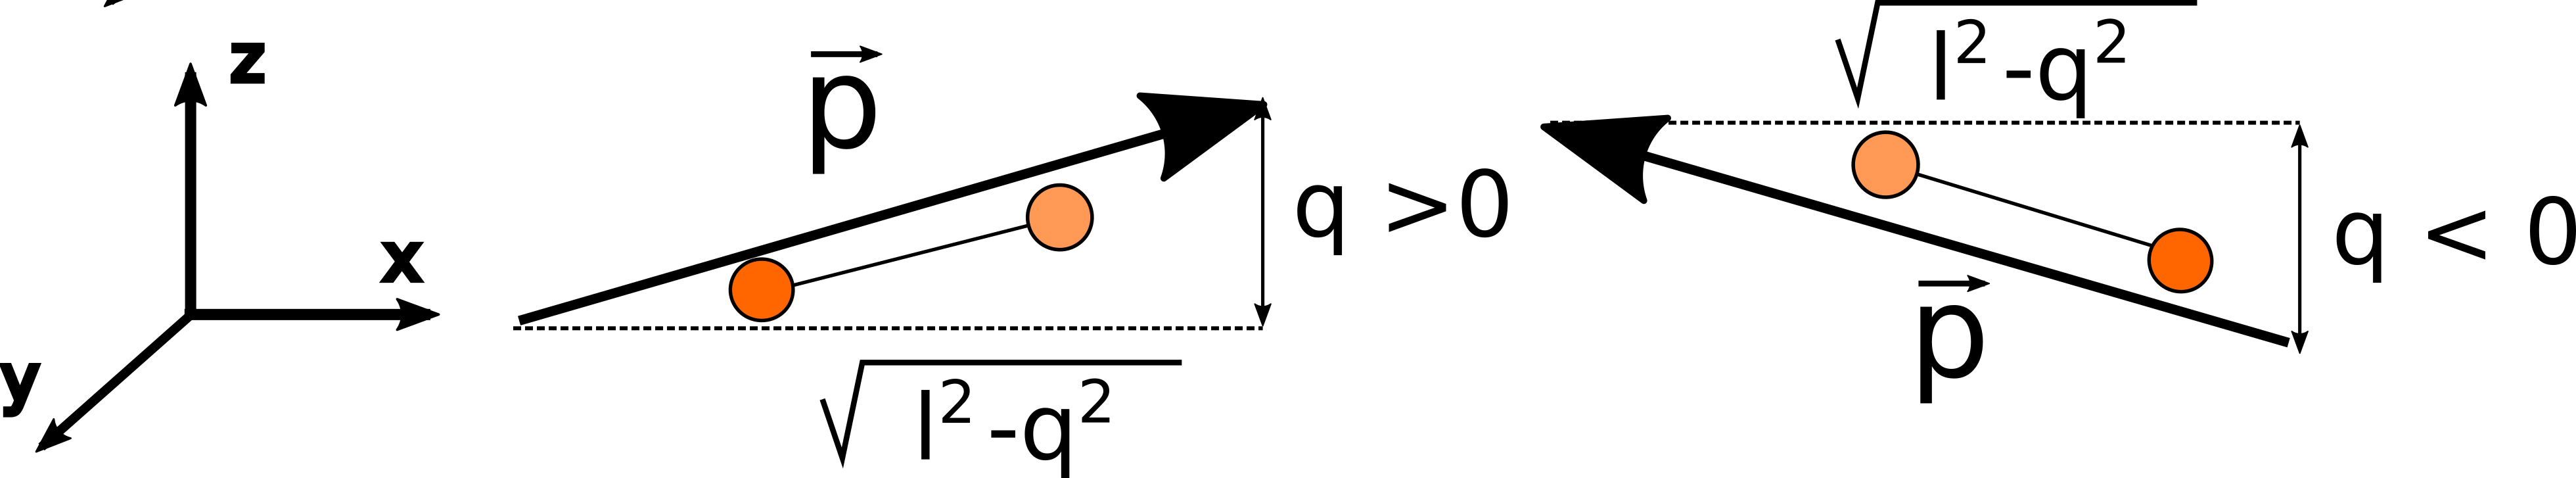
\includegraphics[width=0.8\linewidth]{graphics/DimerQParameterization.png}
			\caption{PLACEHOLDER}
			\label{Fig::DimerMapping}
		\end{figure}
		This is achieved by adding a factor $m = 2$ into the $J_\delta \cos \left(m \Delta \vartheta_{i, j}\right)$ terms. As stated in \autoref{Section::Silicon}, the dimers are buckled by  $18^{\circ}$ corresponding to a an angle $\vartheta^\pm=	\pm 72^\circ \approx	\pm \tfrac{2}{5} \pi $~. The equilibrium positions of \autoref{Eq::XY-Hamilton-Field} are determined by the symmetry breaking field and the parameter $p$ since the interaction is $O(2)$-symmetric. The minima satisfy
		\begin{equation}
			\cos \left(p \vartheta^\pm\right) =	-1~, \qquad \text{implying that} \qquad p \approx 2.57 ~,
		\end{equation} 
		to ensure to reproduce the experimental equilibrium positions. The resulting potential of the symmetry breaking field is shown in \autoref{Fig::XY-Silicon-Potential}. \\		
		\begin{figure}[htp]
			\centering
			\includegraphics[width=0.8\linewidth]{graphics/XY-Silicon-potential.png}
			\caption{The external field in combination with the restriction of $\vartheta$ leads to  the shown potential. The angle is measured from the $(110)$ axis for illustration purposes. The Dynamics of the dimers for sufficiently low temperatures will take place around $\vartheta =	0$, the bucklings of $\vartheta =	\pm \tfrac{1}{2} \pi$ will almost never be reached.}
			\label{Fig::XY-Silicon-Potential}
		\end{figure}
		A suitable order parameter for this model is 
		\begin{equation} \label{Eq::Si-Order-Param}
			M_L =	\frac{1}{L^2} \sum_{i,j} m(\vartheta_{i, j}) \qquad \text{with} \qquad	m(\vartheta) =	\sin \left(\tfrac{p}{2} \vartheta\right) ~,
		\end{equation}
		as the $m(\vartheta)$ have maxima at $\vartheta^{+}$ and minima at $\vartheta^{-}$ satisfying $m(\vartheta^+) =	- m (\vartheta^-)$.
		
		Since in the XY-model the natural conjugated coordinate is the angle $\vartheta$ and therefore the equations of motions \autoref{Eq::Langevin-eq-motion-set-x} have to be adapted to rotary motion. The velocity is replaced by the angle velocity $\alpha$ in this case.
		
		\autoref{Eq::XY-Hamilton-Field} yields the force
		\begin{equation} \label{Eq::Potential-Derivative}
			\begin{split}
							\frac{\partial V(\{\vartheta\})}{\partial \vartheta_{i, j}} = ~~~& J_\parallel m \Big( \sin \left(\vartheta_{i,j} - \vartheta_{i + 1, j} \right) +   \sin \left(\vartheta_{i,j} - \vartheta_{i-1, j} \right) \Big)	 \\
							 + &J_\parallel m \Big( \sin \left(\vartheta_{i,j} - \vartheta_{i, j+1} \right) +  \sin \left(\vartheta_{i,j} - \vartheta_{i, j-1} \right) \Big) \\
							 + &h p \sin(p\vartheta_i)~.
			\end{split}
 		\end{equation}
 		Eventually, the langevin equations to integrate become
 		\begin{align}
 			&\frac{\text{d}}{\text{dt}} \vartheta_{i,j}(t) =	 \alpha_{i,j}(t)~, \\
 			&\frac{\text{d}}{\text{dt}} \alpha_{i,j}(t) =	- \eta \alpha_{i,j}(t) - \frac{\partial V(\{\vartheta\})}{\partial \vartheta_{i,j}} + \sqrt{2 k_B T \eta} \Gamma(t)~,
 		\end{align}
 		with $\frac{\partial V(\{\vartheta\})}{\partial \vartheta_{i,j}}$ given in \autoref{Eq::Potential-Derivative}. The implementation of the solution of this coupled set of stochastic differential equations will be the subject of the next section.
\chapter{Implementation and Results}
	To reduce finite size corrections it is beneficial to consider as large systems as possible. Combined with the critical slowing down described in  \autoref{Section::Dynamic-Scaling} the problem at hand inherently generates an arbitrarily large computational cost. On top comes the stochastic nature of the system, requiring to run many simulations to extract ensemble averages, as well as the need to avoid discretization errors and ensure convergence when implying \autoref{Eq::BBK-method} by choosing a small $dt$. This makes an efficient and fast implementation a crucial part of our investigations.
	\section{GPU programming}
	Besides the difficulties just described, there is an advantage that can be made use of. The langevin equations for the different lattice sites may be coupled through the potential \autoref{Eq::Potential-Derivative}, but the integration step for $t + dt$ only depends of the $\vartheta_{i, j}(t)$ of the previous step, meaning that the integrations can be performed simultaneously. This allows for heavy parallelization, making the problem predestined for a GPU implementation. \\
	
	The main difference between a conventional single core implementation on a central processing unit (CPU) and one on a graphical processing unit (GPU) is the number of processing cores involved. While CPUs only have few ($\sim 10$) powerful processing cores, GPUs are made up of more than $\sim 10^4$ cores. The CPU solves problems in a sequential matter, doing calculation after calculation making it suitable for usecases where the next step directly depends on the on before. In contrast, the GPU is able to perform many independent calculations real time simultaneously on its different cores. In situations where this is applicable, GPU implementations yield a significant speedup of up to a factor of $10^3$. A concept of the different solution approaches is shown in \autoref{Fig::CPU-vs-GPU}.\\
	\begin{figure}[htp]
		\centering
		
\includegraphics[width=0.8\linewidth]{graphics/CPU-vs-GPU.png}
		\caption{A CPU using single core processing would integrate the langevin equation for lattice site $i$ and move on to site $i+1$. The use of multi core processing would allow the CPU to integrate 4 sites simultaneously. In contrast, using GPU programming enables to evaluate the langevin equation at about $10^4 - 10^5$ sites at the same time.}
		\label{Fig::CPU-vs-GPU}
	\end{figure}

	For performance reasons the implementation took place (?) in \texttt{C++} using \texttt{Thrust} \cite{thrust} as high level interface for Nvidia's parallel computing platform \texttt{Cuda} \cite{cuda}. The source code can be found at \texttt{https://github.com/andiw99/Master-Arbeit}. The architecture is inspired by Ahnert et al.'s work \cite{ahnert2014solving}.
	\section{Benchmarks}
	Since an analytic solution of our model is intractable, proper benchmarks are vital to ensure the correctness of our simulation. Furthermore the stepsize used in \autoref{Eq::BBK-method} has to be analyzed to ensure convergence as well as a balance between the discretization error and efficiency.
	
	The Benchmarks that were conducted are   
	\begin{itemize}
		\item the statistics of independent harmonic oscillators with thermal coupling,
		\item the equilibrium distribution of particles in a cosine potential,
		\item the equilibrium distribution of a system composed of two particles in a cosine potential with cosine interaction
	\end{itemize}			
	The equation that describes the time evolution of probability densities of brownian motion is the \textbf{Fokker-Planck equation}. When talking about the probability density $p(x, v, t)$ in terms of particle velocity $v$ and position $x$ it is often referred to as the \textbf{Klein-Kramers-} or \textbf{Smoluchowski} equation and written as
	\begin{equation} \label{Eq::Klein-Kramers}
	\frac{\partial}{\partial t} p(x, v, t) = \left(-\frac{\partial}{\partial x} v + \frac{\partial}{\partial v} \left(\eta v - \frac{1}{m} \frac{\partial}{\partial x} V(x) \right) + \frac{\eta k_B T}{m} \frac{\partial}{\partial v^2}\right)p(x, v, t) ~.
	\end{equation}
	The Fokker-Planck equation and the langevin equations (\autoref{Eq::Langevin-eq-motion-set-x} and \autoref{Eq::Langevin-eq-motion-set-p}) are virtually identical and can be converted into each other. Ensemble averages over paths of langevin equations result in the probability distribution satisfying \autoref{Eq::Klein-Kramers}. The steady state distribution of the Fokker-Planck equation is the canonical distribution
	\begin{equation} \label{Eq::Canonical-Dist}
		p(x, v) \propto e^{\beta \left( \tfrac{1}{2} m v^2 + V(x)\right)},	
	\end{equation}
	allowing for an easy way to verify long term behavior.  
	\subsection{Thermal harmonic oscillators}
	For a quadratic potential 
	\begin{equation}
		V(x) =	\tfrac{1}{2} \omega^2 x^2,
	\end{equation}
	the Fokker-Planck equation is analytically solvable \cite{risken1996fokker}. This makes it ideal to confirm correct dynamics of the simulation. The analytic solution for the second moment of $x(t)$ reads
	\begin{equation}
		\left \langle x^2 \right \rangle (t)  =	\frac{\eta {k_B T}}{m (\lambda_+ - \lambda_-)^2} \left[ \frac{\lambda_+ + \lambda_-}{\lambda_+ \lambda_-} + \frac{4}{\lambda_+ + \lambda_-} \left(e^{- (\lambda_+ + \lambda_-) t} - 1\right) - \frac{1}{\lambda_+} e^{-2\lambda_+ t} - \frac{1}{\lambda_-} e^{- 2 \lambda_- t}\right],
	\end{equation}
	with 
	\begin{equation}
		\lambda_{\pm} =	\frac{1}{2} \left(\eta \pm \sqrt{\eta^2 - 4 \omega^2}\right)
	\end{equation}
	In \autoref{Fig::MSD-Comparison} we compare $\left \langle x^2 \right \rangle (t)$ calculated from $\approx65000 $ path, simulated by either the Euler-Maruyama- or the BBK method, with the theoretical result. The BBK algorithm with $dt =	0.05$ and the Euler-Maruyama method with $dt =	0.001$ yield similar small deviations from the theoretical curve, suggesting that the BBK method can be used up to much larger stepsizes. Besides, the validity of both methods for thermal harmonic oscillators is given for both methods for small enough stepsizes.

	\begin{figure}[htp]
		\begin{subfigure}{0.5\textwidth}
			\centering
			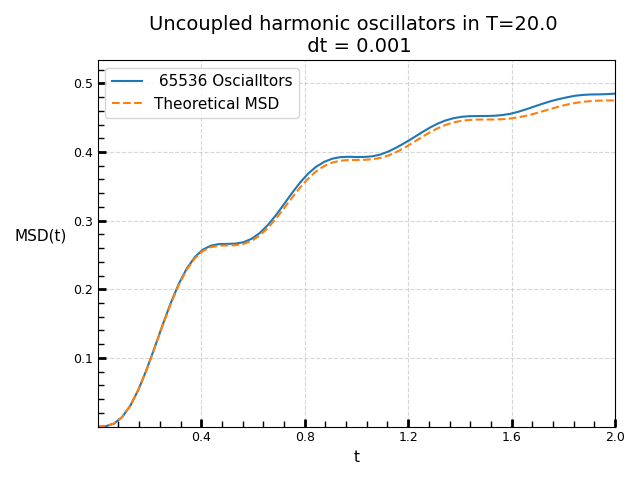
\includegraphics[width=0.8\linewidth]{graphics/MSD-Euler-0.001.png}
			\caption{The Euler-Maruyama method with a stepsize of $dt=0.001$ results in small but noticeable deviations.}
		\end{subfigure}
		\begin{subfigure}{0.5\textwidth}
			\centering
			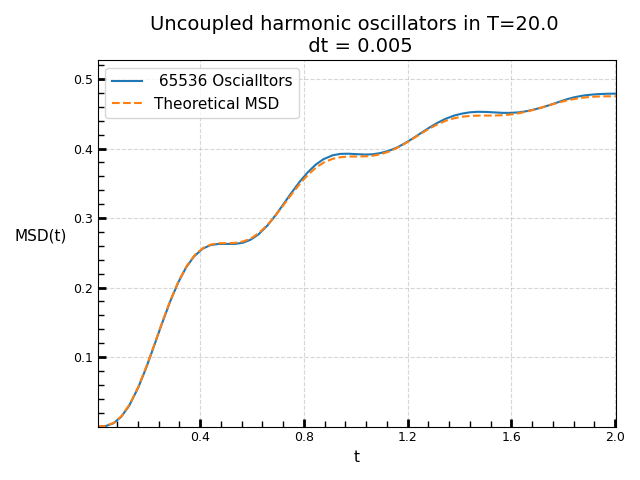
\includegraphics[width=0.8\linewidth]{graphics/MSD-BBK-0.005.png}
			\caption{The BBK method with a stepsize of $dt=0.005$ reproduces the theoretical curve very well.}
		\end{subfigure}  \\
		\begin{subfigure}{0.5\textwidth}
			\centering
			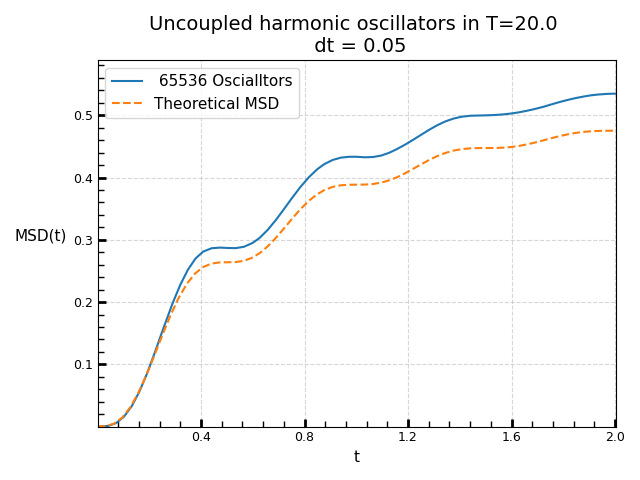
\includegraphics[width=0.8\linewidth]{graphics/MSD-Euler-0.05.png}
			\caption{The Euler-Maruyama method with a stepsize of $dt=0.05$ results in large deviations.}
		\end{subfigure}
		\begin{subfigure}{0.5\textwidth}
			\centering
			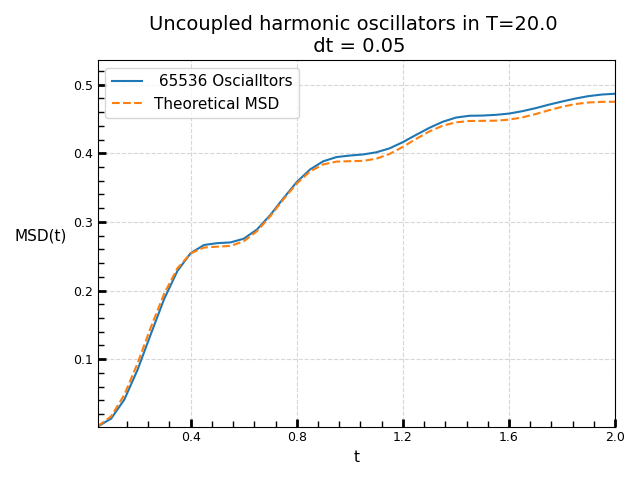
\includegraphics[width=0.8\linewidth]{graphics/MSD-BBK-0.05.png}
			\caption{The BBK method with a stepsize of $dt=0.05$ results in small but noticeable deviations.}
		\end{subfigure}
		\caption{The calculated $\left \langle x^2 \right \rangle (t)$ of thermal harmonic oscillators are compared for the Euler-Maruyama- and the BBK method with different stepsizes}
		\label{Fig::MSD-Comparison}
	\end{figure}
	
	\subsection{Particles in a cosine potential}
	Another valuable Benchmark is the edge case of weakly interacting particles with $J=0$. We will confirm that probability distribution calculated from  $???$ particle paths will approach the theoretical equilibrium distribution given by inserting \autoref{Eq::XY-Hamilton-Field} for $J_\delta =	0$ into \autoref{Eq::Canonical-Dist}. \\
	
	In \autoref{Fig::Cos-Prob-Dist} we show the calculated integrated probability density $p(x) =	\int_{}^{} p(x, v) dv$ is plotted. The BBK method shows virtually no discretization errors up to a stepsize of $dt =	0.05$. For the Euler-Maruyama method large discretization errors show up for stepsizes one magnitude smaller. \\
	
	Again, for sufficiently small stepsizes the long term behavior of our simulation is  verified. 
	
	\begin{figure}[htp]
		\begin{subfigure}{0.5\textwidth}
			\centering
			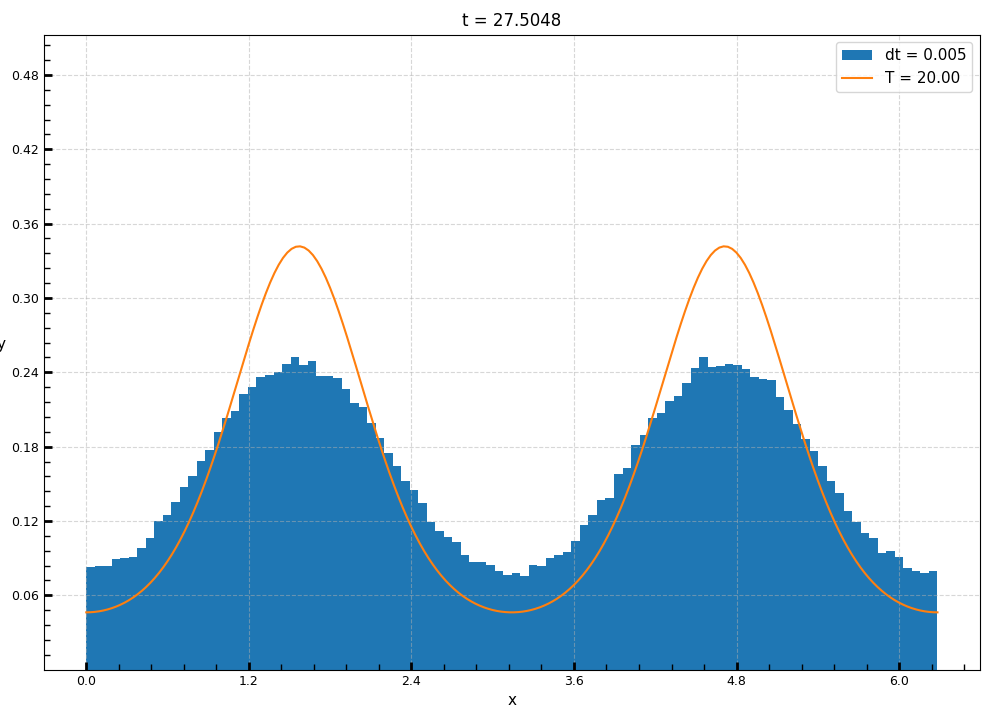
\includegraphics[width=0.8\linewidth]{graphics/Distribution-Euler-0.005.png}
			\caption{The Euler-Maruyama method shows significant discretization errors regarding $p(x)$ even for a comparatively small stepsize of $dt =	0.005$.}
		\end{subfigure}
		\begin{subfigure}{0.5\textwidth}
			\centering
			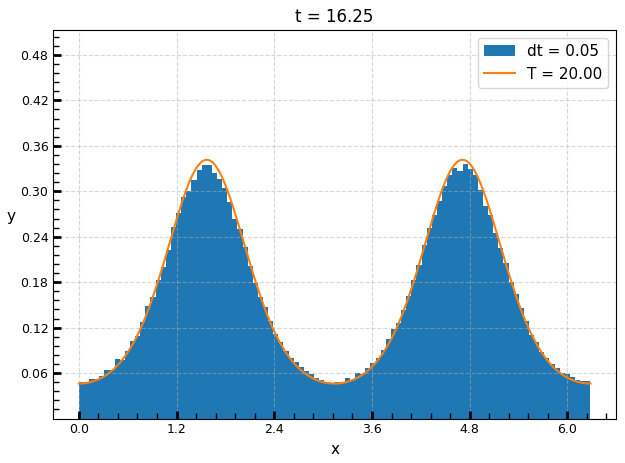
\includegraphics[width=0.8\linewidth]{graphics/Distribution-BBK-0.05.png}
			\caption{The BBK method shows almost no deviation from the theoretical $p(x)$ even for a stepsize of $dt =	0.05$.}
		\end{subfigure}
		\caption{The integrated probability distributions $p(x)$ calculated from ??? particle paths are compared to the theoretical equilibrium distribution for the Euler-Maruyama method and the BBK Algorithm. It was made sure that the systems were completely relaxed, meaning that the effects of the starting position vanished and the shape of the probability distribution did not change anymore.}
		\label{Fig::Cos-Prob-Dist}
	\end{figure}
		
	\subsection{Two interacting particles in a cosine potential}
	The third benchmark has the purpose of verifying the correct behavior of the interaction. Since the equilibrium distribution becomes a high dimensional function $p(\{x_i\}, \{v_i\})$, a suitable representation is possible in the case of system consisting of two particles. The object of examination is again the equilibrium probability distribution of the Fokker-Planck equation.\\
	
	In \autoref{Fig::Pair-Prob-Dist} we now show cuts of the integrated probability density $p(x_1, x_2) =	\int_{} p(x_1, x_2, v_1, v_2) dv_2 dv_1$ with a constant $x_2$. It is verified that simple interacting systems are driven to their equilibrium by the method of langevin integrations. The statistical- and discretization errors vanish for many samples and small stepsizes.
	
		\begin{figure}[htp]
		\begin{subfigure}{0.5\textwidth}
			\centering
			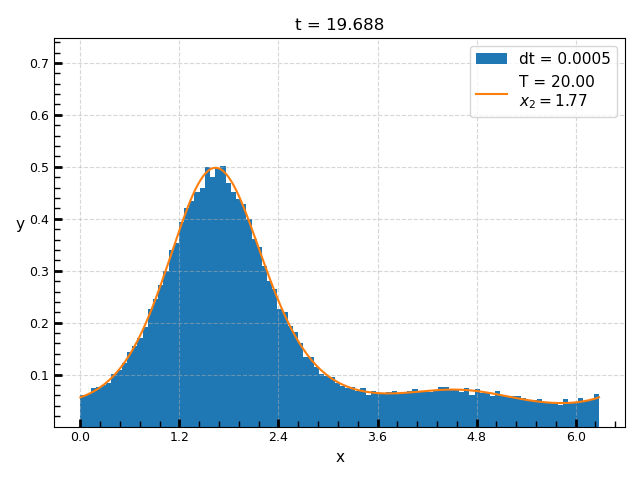
\includegraphics[width=0.8\linewidth]{graphics/Pair-Equil-Dist-20.png}
			\caption{Different x2s?}
		\end{subfigure}
		\begin{subfigure}{0.5\textwidth}
			\centering
			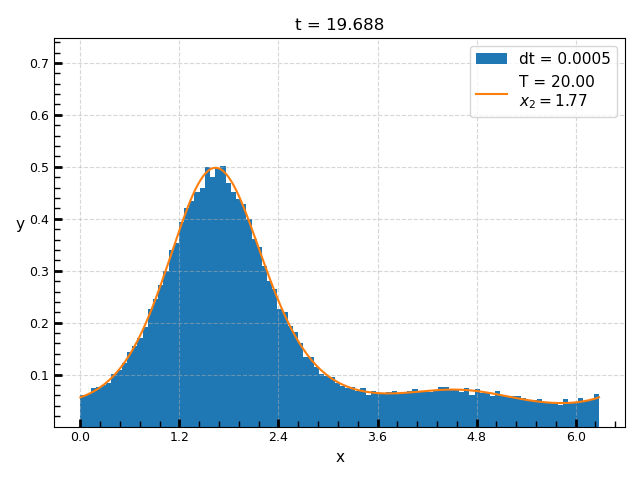
\includegraphics[width=0.8\linewidth]{graphics/Pair-Equil-Dist-20.png}
			\caption{Different Temperatures?}
		\end{subfigure}
		\caption{Cuts of the integrated probability distributions $p(x_1, x_2)$ with a constant $x_2$ calculated from ??? particle paths are compared to the theoretical equilibrium distribution. It was made sure that the systems were completely relaxed, meaning that the effects of the starting position vanished and the shape of the probability distribution did not change anymore.}
		\label{Fig::Pair-Prob-Dist}
	\end{figure}
	
	\section{Results}
		In the following the results of the explained simulation will be presented. We will start with the examination of the critical exponents of our model. \\
		
		The parameters will be measured in units of $J_\perp =	1$ and the initially used ratio $J_\parallel /	J_\perp =	31.1$ is the one from Brand et. al \cite{brand2023dimer}. The external field $h =	5$ is chosen small compared to $J_\parallel$ to ensure approximate validity of \autoref{Eq::Crit-Temp-XY}. The strength of $h$ should not influence the kind of phase transition we observe as long as it is finite, but may influence $T_c$. Both coupling strengths are negative to reproduce the c(4x2) symmetry. To conclude, as long as not otherwise stated, the in the following used model parameters of \autoref{Eq::XY-Hamilton-Field} are
		\begin{equation}
			J_\perp =	-1~, \qquad \qquad J_\parallel =	-31.1 \qquad \text{and} \qquad h =	5.
		\end{equation}
		The dampening is set to $\eta =	1.5$. Our method of correlation length extraction \autoref{Section::Corr-Lenght-Calculation} works best if $\xi_\delta \ll L_\delta$. Since the Si(001) surface exhibits a large correlation length anisotropy $\tfrac{(\xi_\parallel /	a_\parallel)}{(\xi_\delta /	a_\delta)} \approx 10 $, it is useful to ensure that the system sizes share a similar ratio. This way we can analyze larger correlation lengths without increasing the computational cost. The following systems have a ratio of $\tfrac{L_\parallel}{L_\perp} =	8$ if not stated otherwise. The used stepsize is $dt = 0.01$
		\subsection{static scaling}
			Since the phase transition of the Si(001) surface seems to belong to the Ising universality class \cite{brand2023critical}, our simulation should reproduce this. The XY model with a $p$-fold symmetry breaking external field belongs to the Ising universality class for $p=2$ \cite{jose1977renormalization}, but the question remains if this is still true for our adaptation (\autoref{Sec::XY-to-Silicon}) with a rational number $p \approx 2.57$. \\
			
			Therefore, the finite size techniques and the Binder cumulant described in \autoref{Section::FSS} and \autoref{Sec::Binder-Cumulant} are employed to extract the critical exponent. The magnetization is calculated using \autoref{Eq::Si-Order-Param}. We initialize totally ordered systems as suggested in \cite{binder2022monte}, that is all dimers are alternatively buckled. We run multiple small independent systems simultaneously on a single GPU to achieve optimal parallelization. We run long simulations to ensure the thermalization of the systems. During the run, we document the Binder cumulant $U_L(t)$ to be able to afterwards determine a timepoint $t_{equil}$ after which we judge the cumulant to be equilibrated. The cumulant is subject to statistical fluctuations, so to obtain useful averages it can be made use of the ergodic hypotheses. Instead of running many simulations and averaging the latest value of $U_L$, we simulate systems for long times $t_{long}$ and calculate the ensemble average as the time average
			\begin{equation}
				\overline{U}_L =	\frac{1}{(t_{long} - t_{equil})} \int_{t_{equil}}^{t_{long}} U_L(t) dt~.
			\end{equation}
			In \autoref{Fig::Binder-Cum-Result} the results for ??? systems simulated until $t_{long} = ???$ are shown for temperatures very close to $T_c$. The critical point was approached by estimating the critical temperature with \autoref{Eq::Crit-Temp-XY} yielding $T_c^{est} \approx 0.618$, examining the general area for the phase transition and then iteratively closing in. The more precise $T_c$ shall be determined, the closer the temperatures have to lie at $T_c$. The closer two temperatures lie, the easier it is for statistical fluctuations to smear their relative position and therefore the more averages you need. The same is true for the calculation of the critical exponent $\nu$. The derivative $\tfrac{\partial U_L}{\partial \varepsilon}$ is calculated through a simple central difference. Afterwards the function \autoref{Eq::FSS-dU_dT} is fitted to $\tfrac{\partial U_L}{\partial \varepsilon} (L)$. The result $\nu =	1.04$ is in good agreement with the theoretical critical exponent of the Ising model $\nu =	1$.
			\begin{figure}[htp]
				\begin{subfigure}{0.5\textwidth}
					\centering
					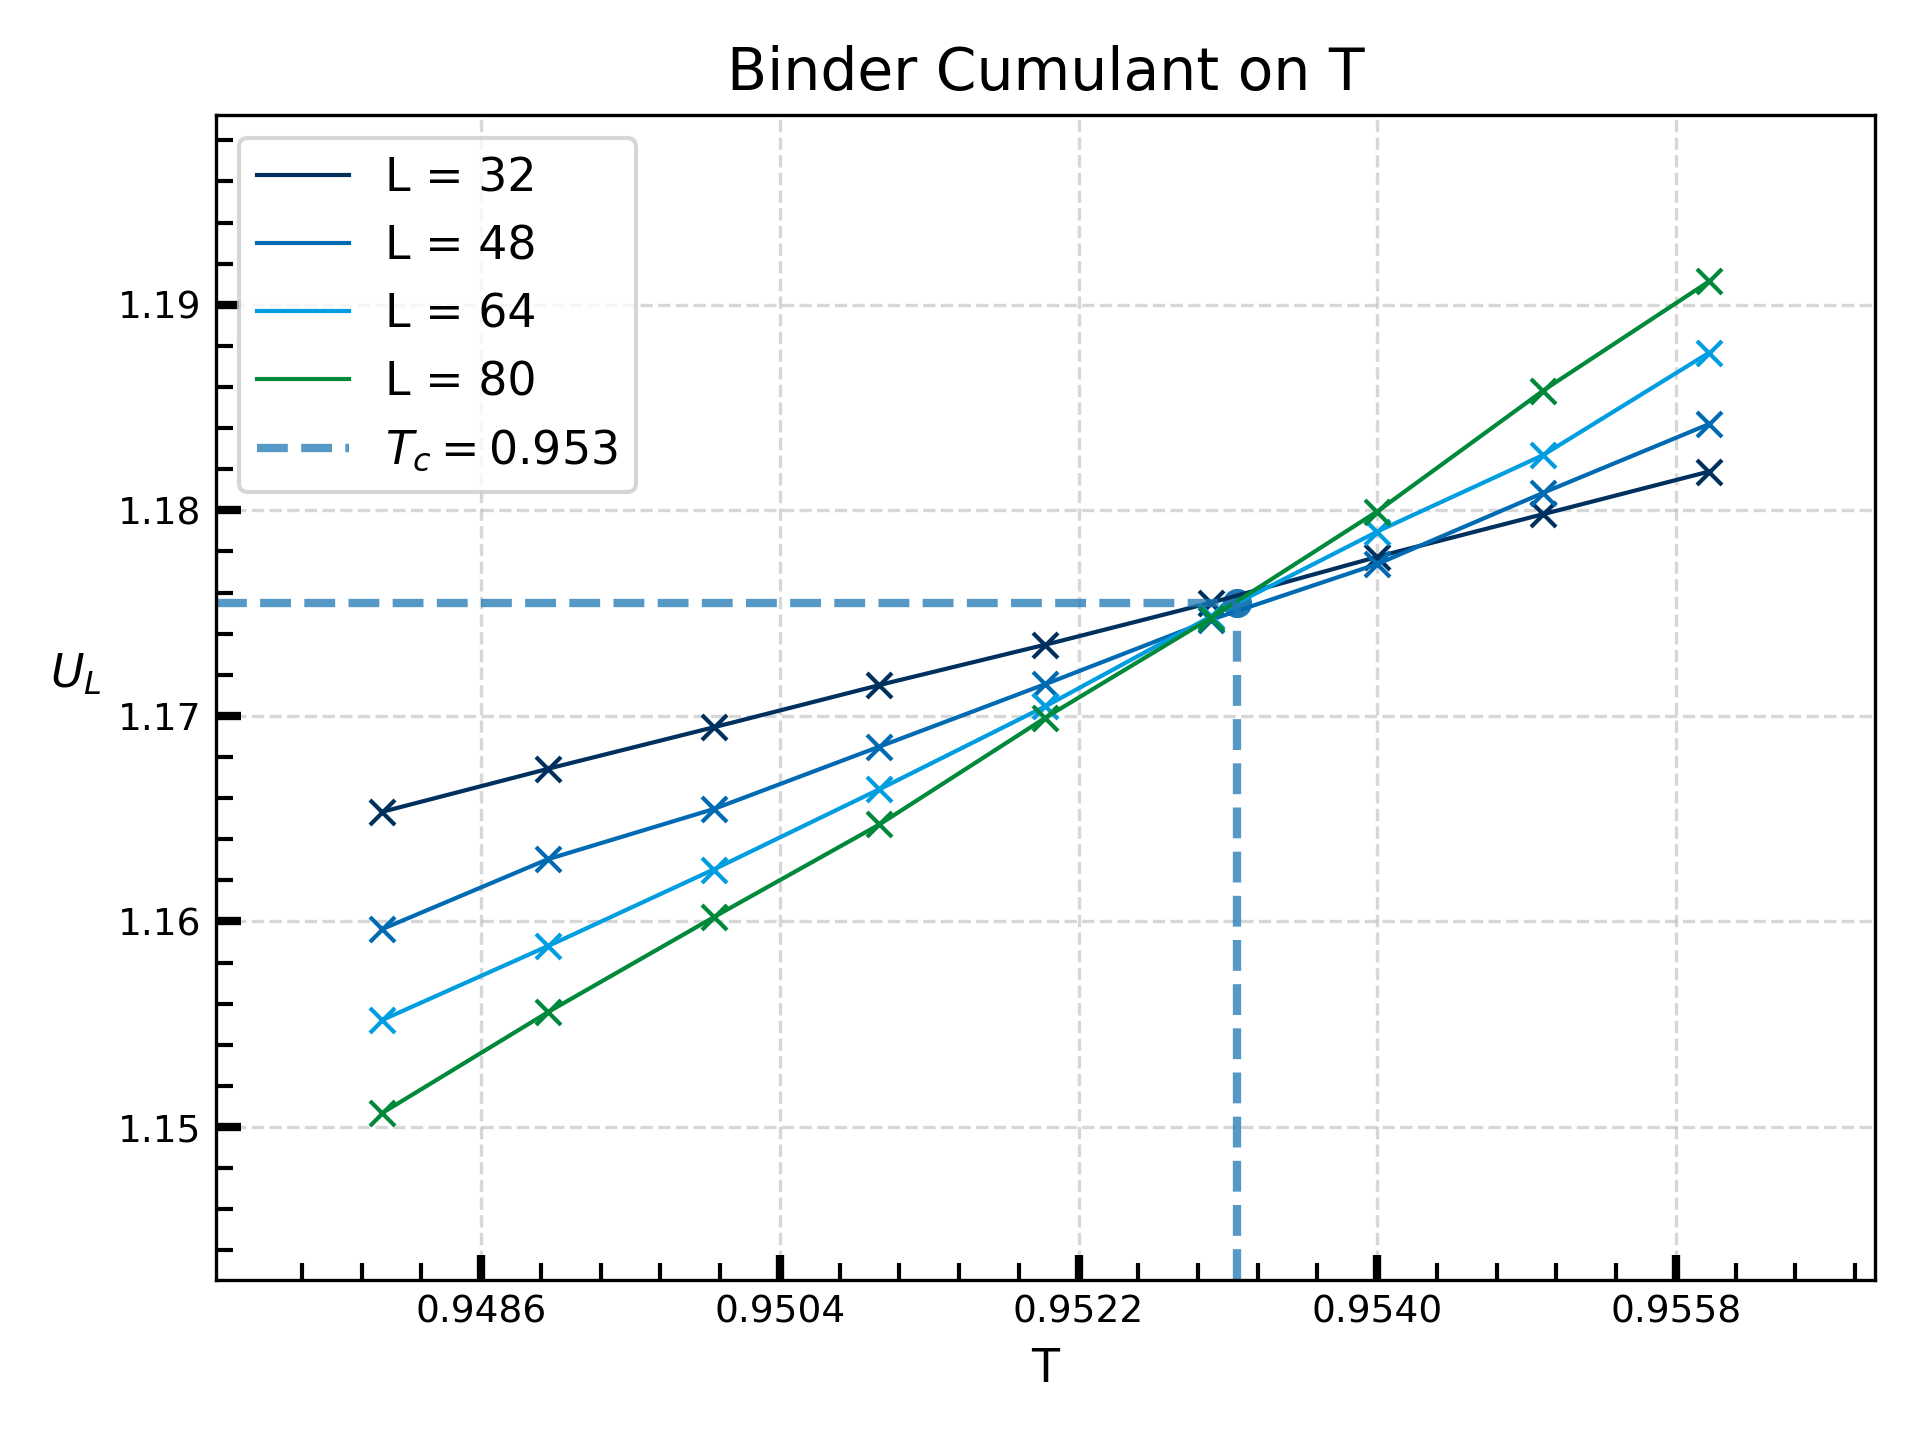
\includegraphics[width=0.8\linewidth]{graphics/cum_time_avg.png}
					\caption{The Binder cumulants intersect at $T_c =	0.953$. The intersection is determined by the minimum squared error between the cumulants.}
				\end{subfigure}
				\begin{subfigure}{0.5\textwidth}
					\centering
					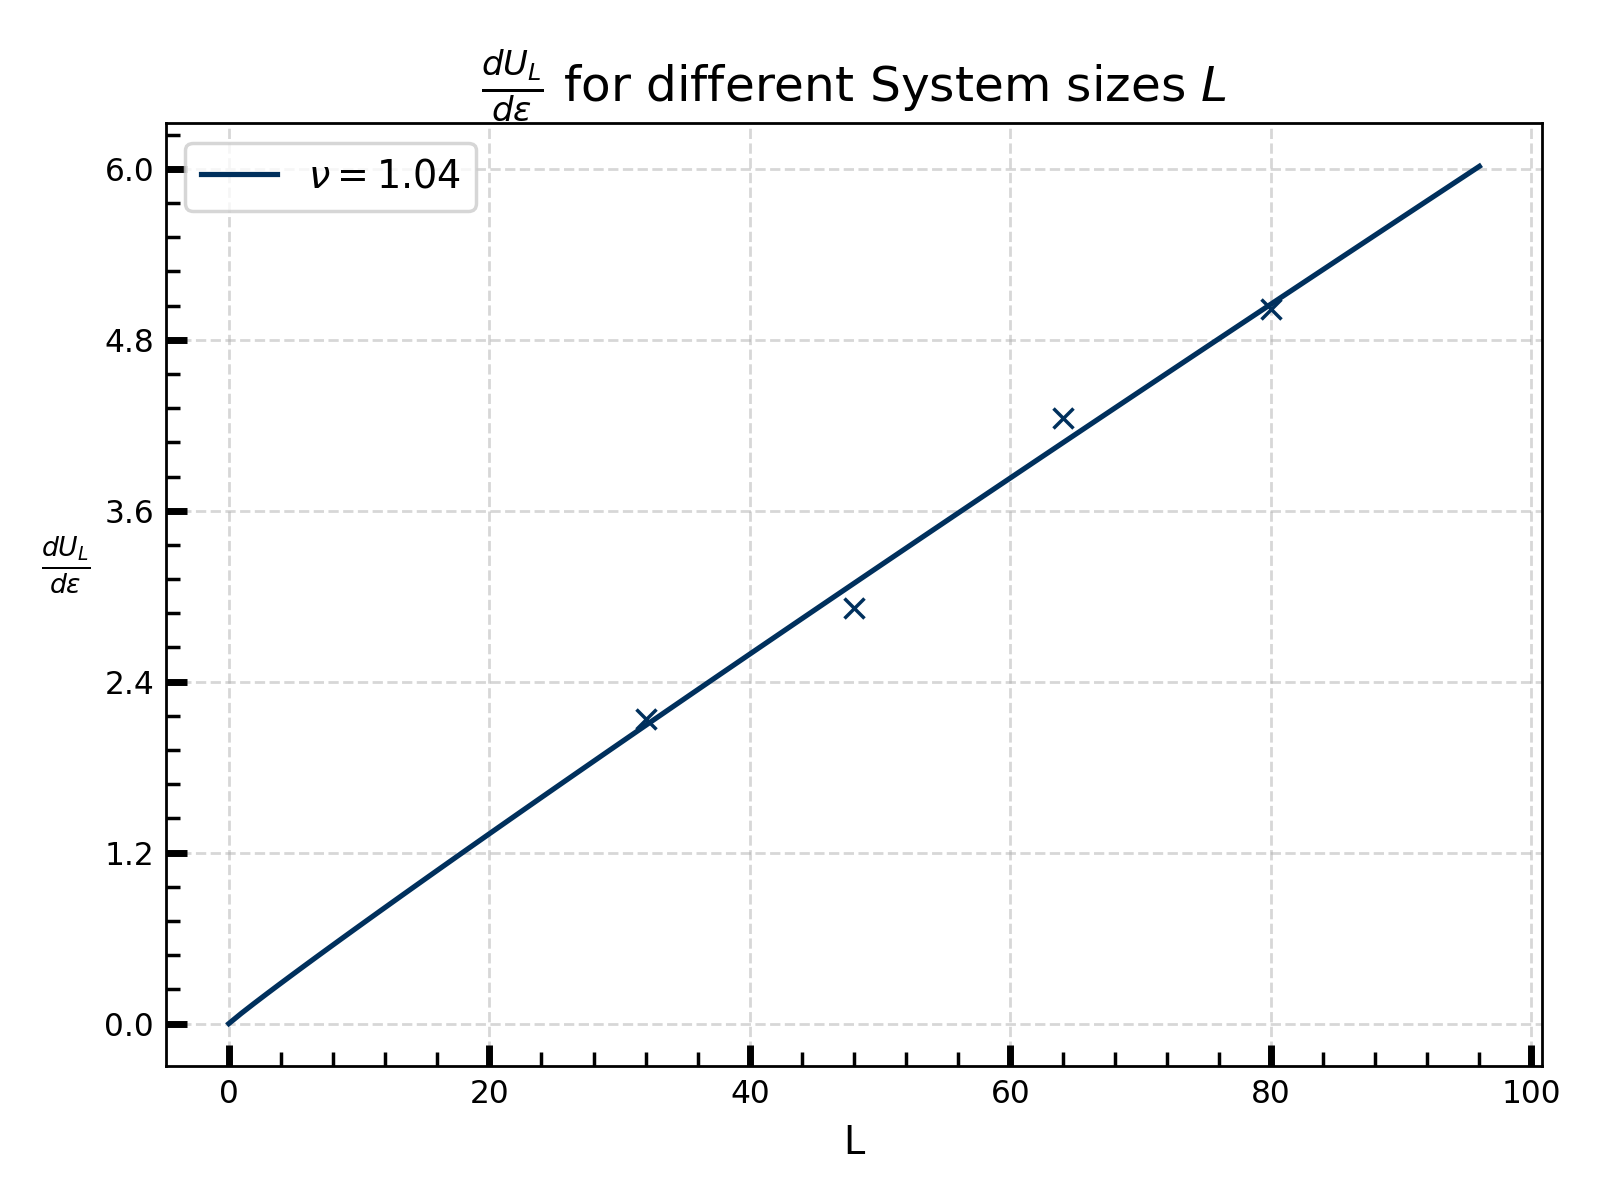
\includegraphics[width=0.8\linewidth]{graphics/critical_exponent_time_avg.png}
					\caption{The derivatives $\frac{\partial U_L}{\partial \varepsilon}$ scale like $\propto L^\nu$. The fitting results in $\nu = 1.04$ which is in good accordance with the Ising model.}
				\end{subfigure}
				\caption{The results for $\overline{U}_L$ of ??? averaged systems of different sizes simulated for a time of $t_{long} =	??? $ are shown. The estimated equilibration time is $t_{equil} =	??? $.}
				\label{Fig::Binder-Cum-Result}
			\end{figure}  
		The matching of the static critical exponent verifies our numerics as well as the assumption that our modification of the XY model still belongs to its expected universality class.
		\subsection{dynamic scaling}
		The dynamic universality classes are subgroups of the static universality classes and our model could very well be in a different dynamic universality class than the 2D Ising model. In the following multiple methods will be employed to extract the dynamic critical exponent $z$. 
		
		\subsubsection{The Kibble-Zurek mechanism}
		The first method will be the extraction through \autoref{Eq::KZM-scaling} and the Kibble-Zurek mechanism. Since we already gained knowledge of $\nu$ we can fit the exponent $\nu /	(1 + \nu z)$ to quenched correlation lengths deduce $z$. \\
		
		The used quench protocol, i.e the manner in which the system is cooled down, will be a simple isotropic, linear quench like \autoref{Eq::Linear-Quench}. The starting temperature $\varepsilon(t_{start})$ is chosen to be sufficiently far away to observe adiabatic system evolution before crossing the freezeout point $\varepsilon(t_{start}) < \varepsilon(\hat{t})$. The end temperature $\varepsilon(t_{end})$ is chosen in symmetric distance from the transition point $|\varepsilon(t_{start})|=|\varepsilon(t_{end})|$. \\
		
		In \autoref{Fig::Quench-Result} the results for the quench of our system are shown. A fit of the frozen correlation lengths $\hat{\xi}$ to \autoref{Eq::KZM-scaling} is performed in \autoref{Fig::Quench-Result-c} and \autoref{Fig::Quench-Result-d}. Only the datapoints in the phase space where the Kibble-Zurek mechanism should be valid are used. It was made sure that $\hat{\xi}_\delta \ll L_\delta$ so that \autoref{Section::Corr-Lenght-Calculation} is still applicable. The extracted KZM exponent of $\nu /( 1 + \nu z)$ is unusually large and suggests that $z < 2$. \\
		
		A KZM independent z extraction method is needed to verify the correct critical exponent. 				
		\begin{figure}[htp]
			\begin{subfigure}{0.5\textwidth}
				\centering
				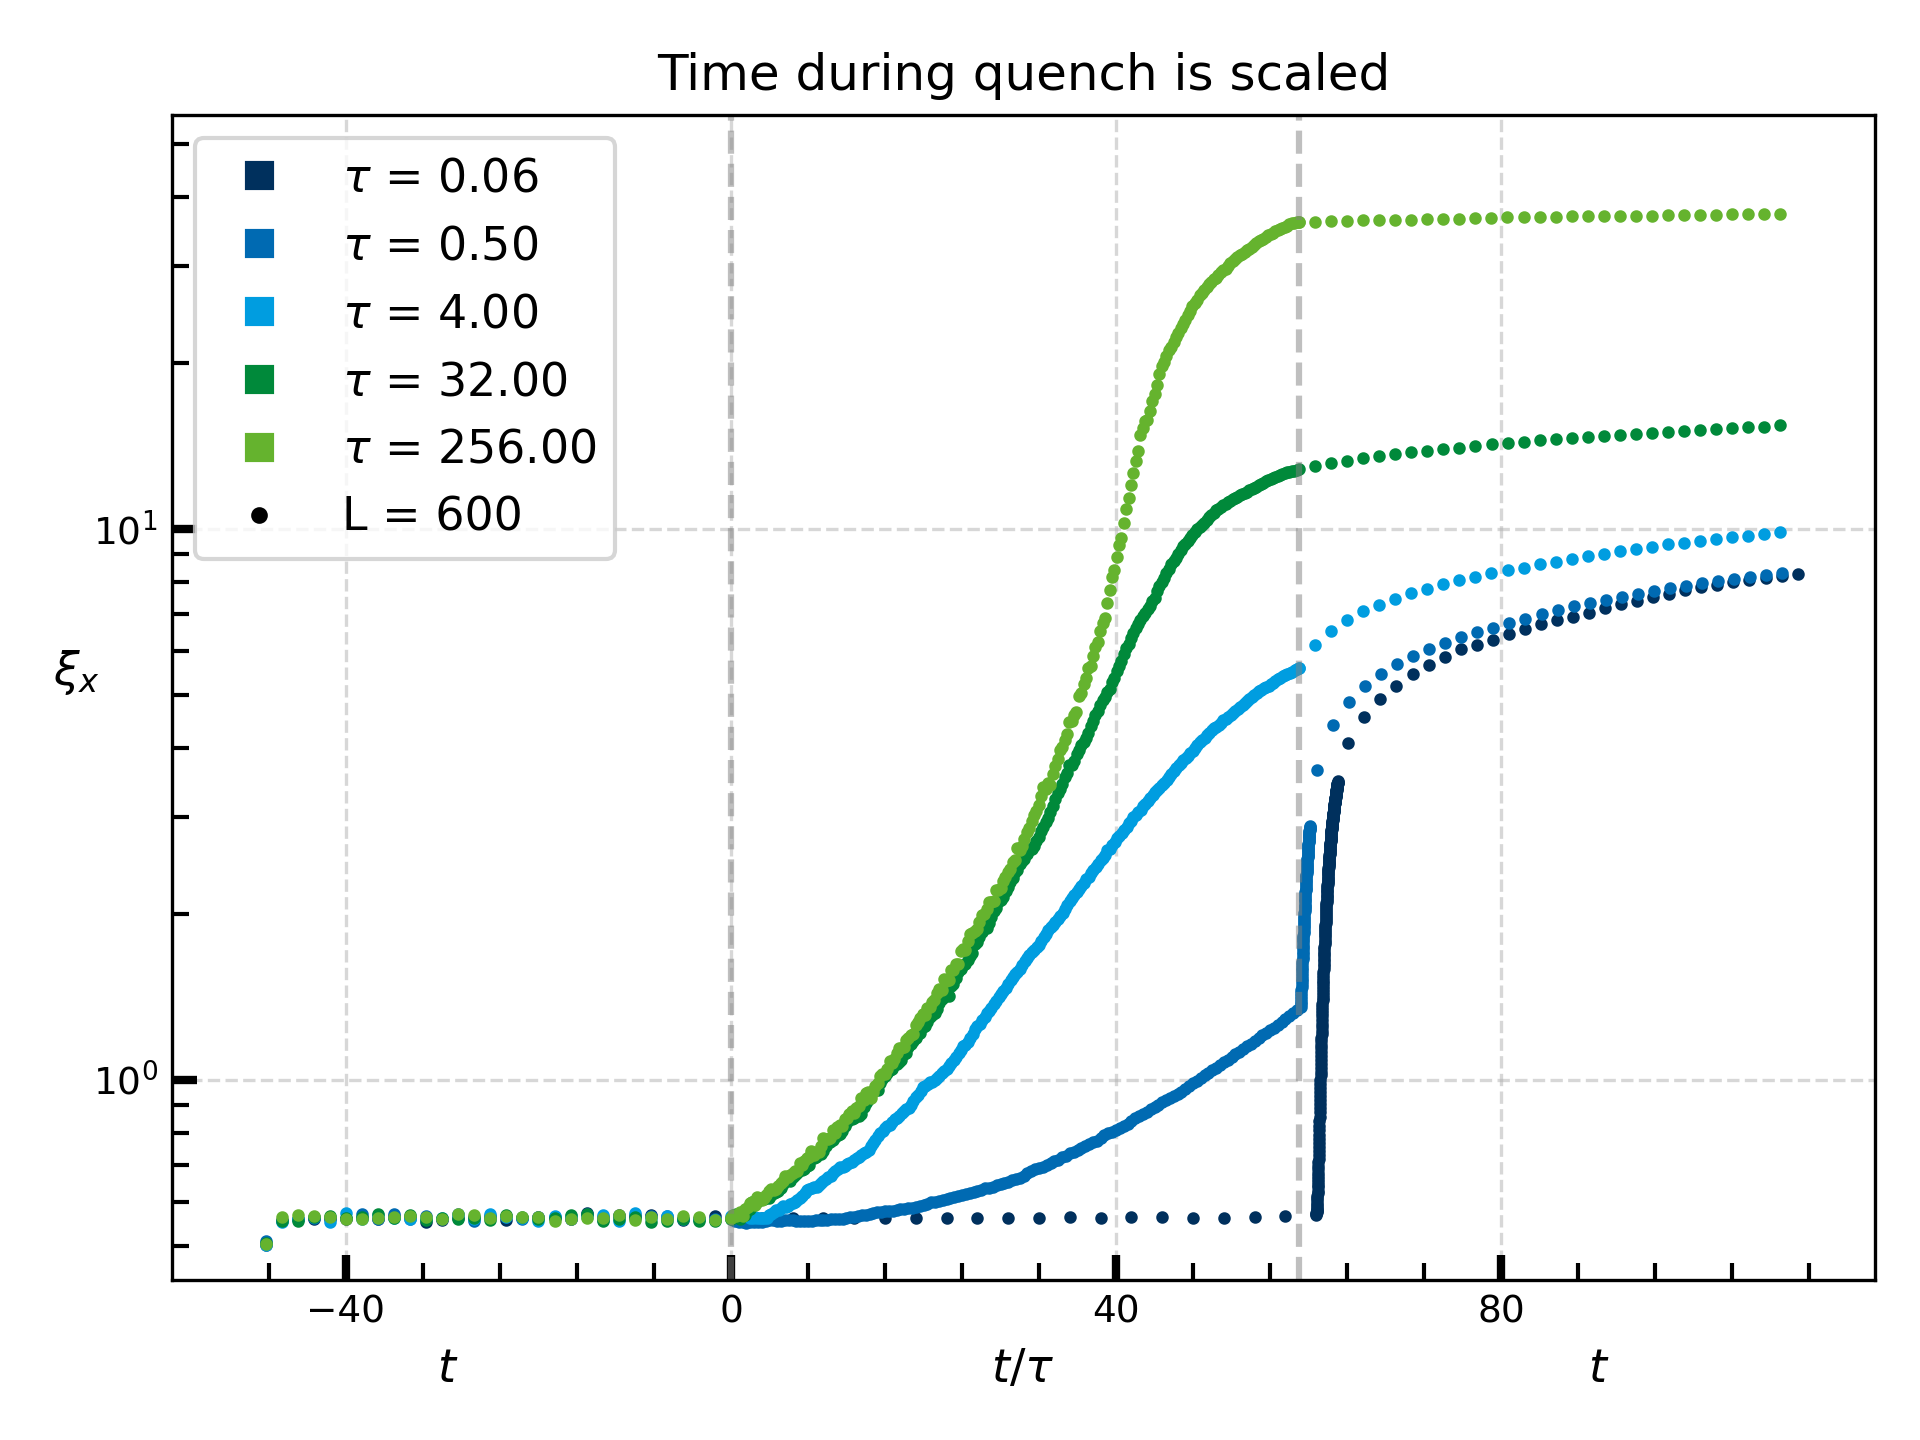
\includegraphics[width=0.8\linewidth]{graphics/xix-process.png}
				\caption{The time-resolved quench-process $\xi_x(t)$ for different quench timescales is shown for the system sizes $L_x =	600, 1200$.}
			\end{subfigure}
			\begin{subfigure}{0.5\textwidth}
				\centering
				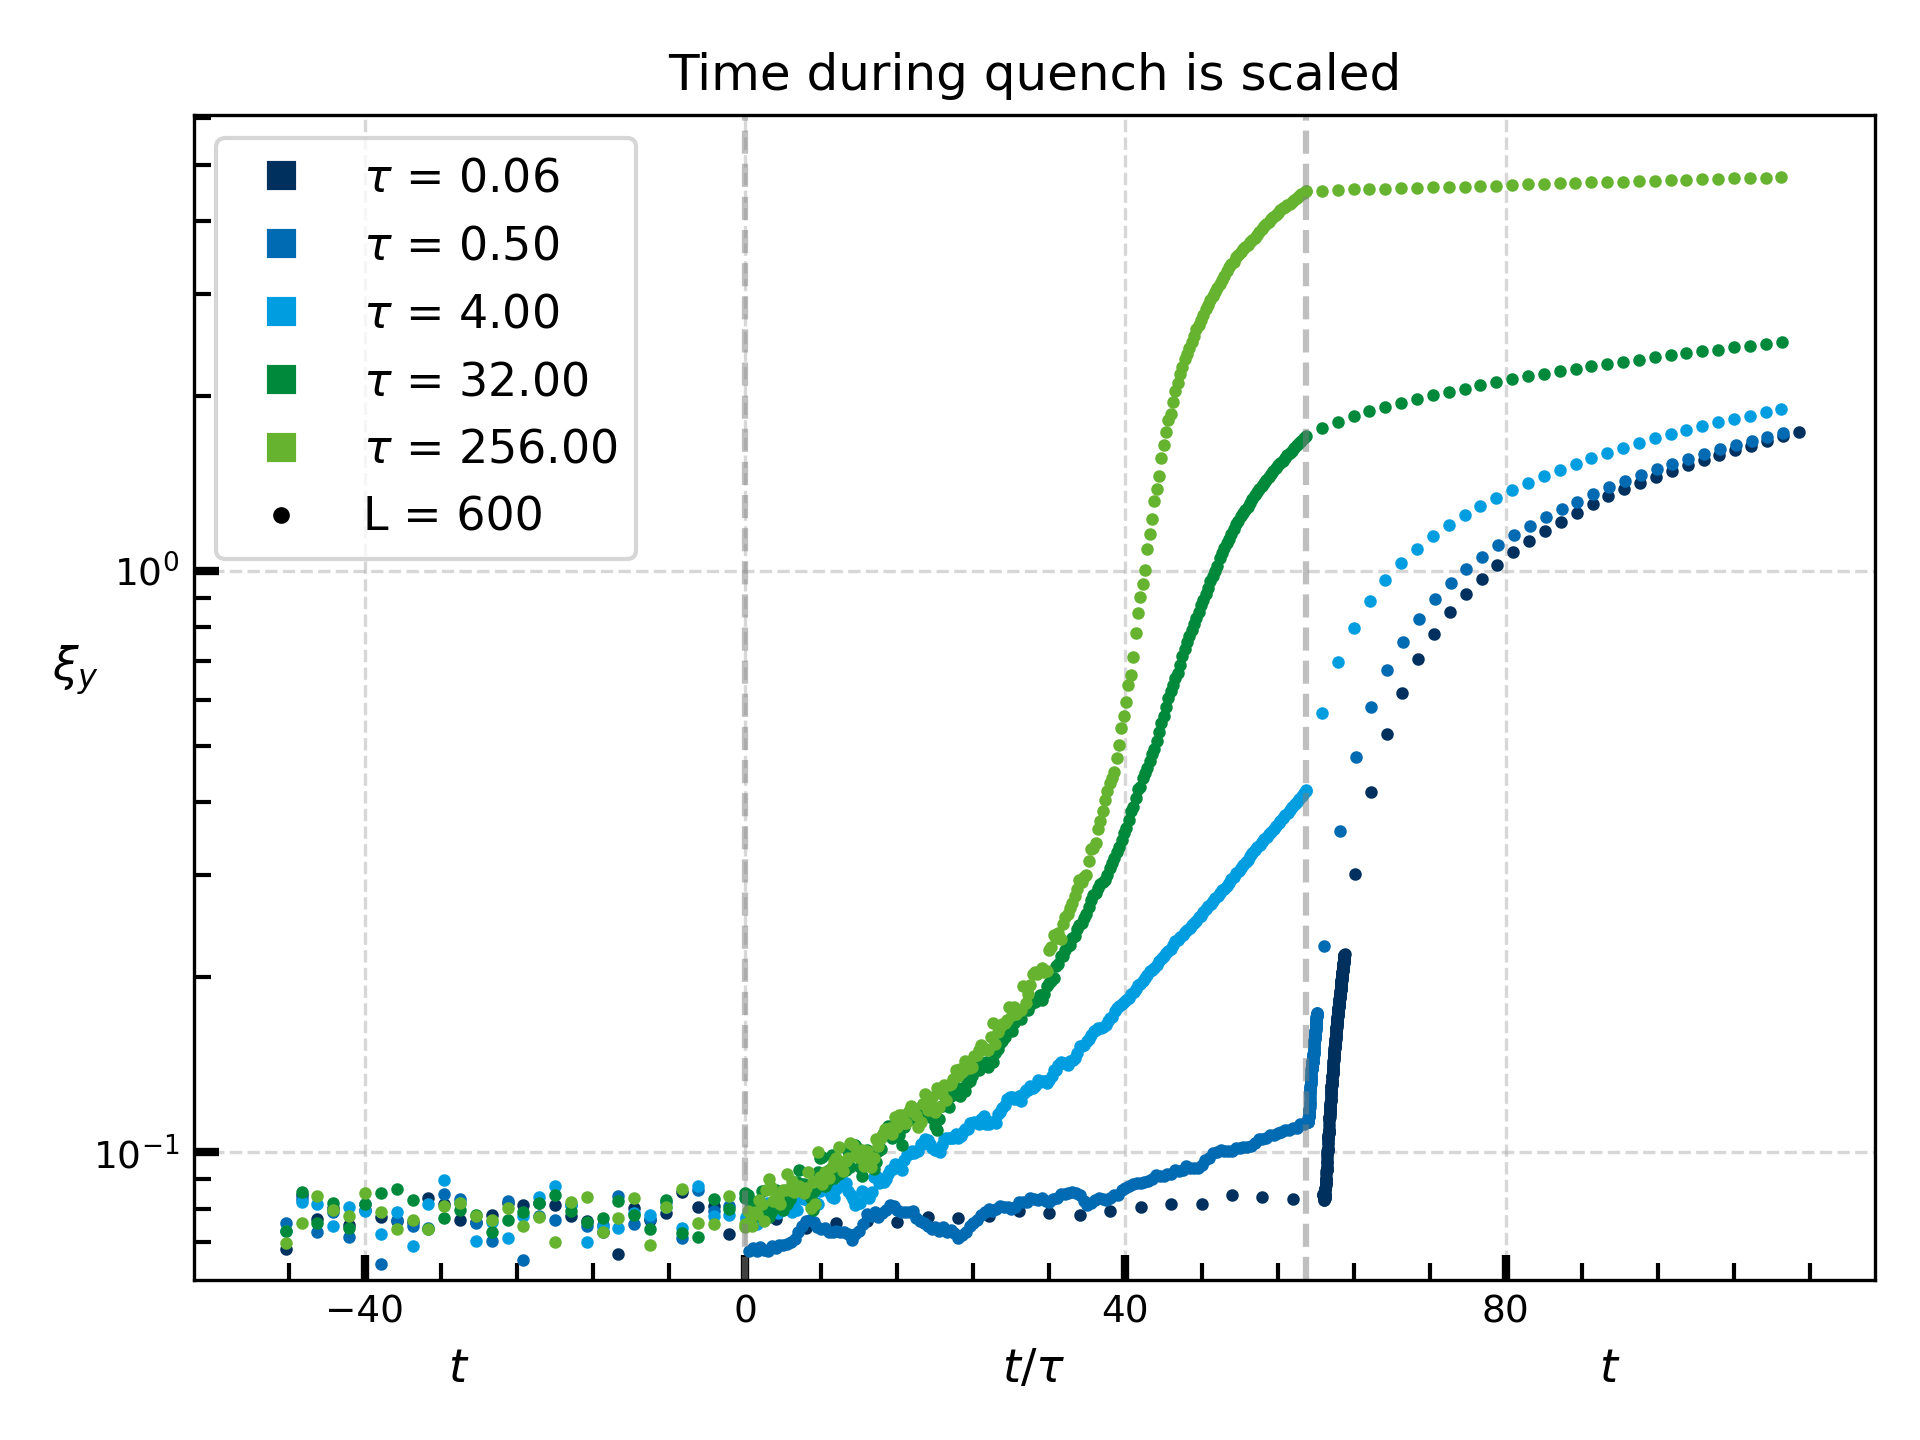
\includegraphics[width=0.8\linewidth]{graphics/xiy-process.png}
				\caption{The time-resolved quench-process $\xi_x(t)$ for different quench timescales is shown for the system sizes $L_y =	75, 150$.}
			\end{subfigure} \\
			\begin{subfigure}{0.5\textwidth}
				\centering
				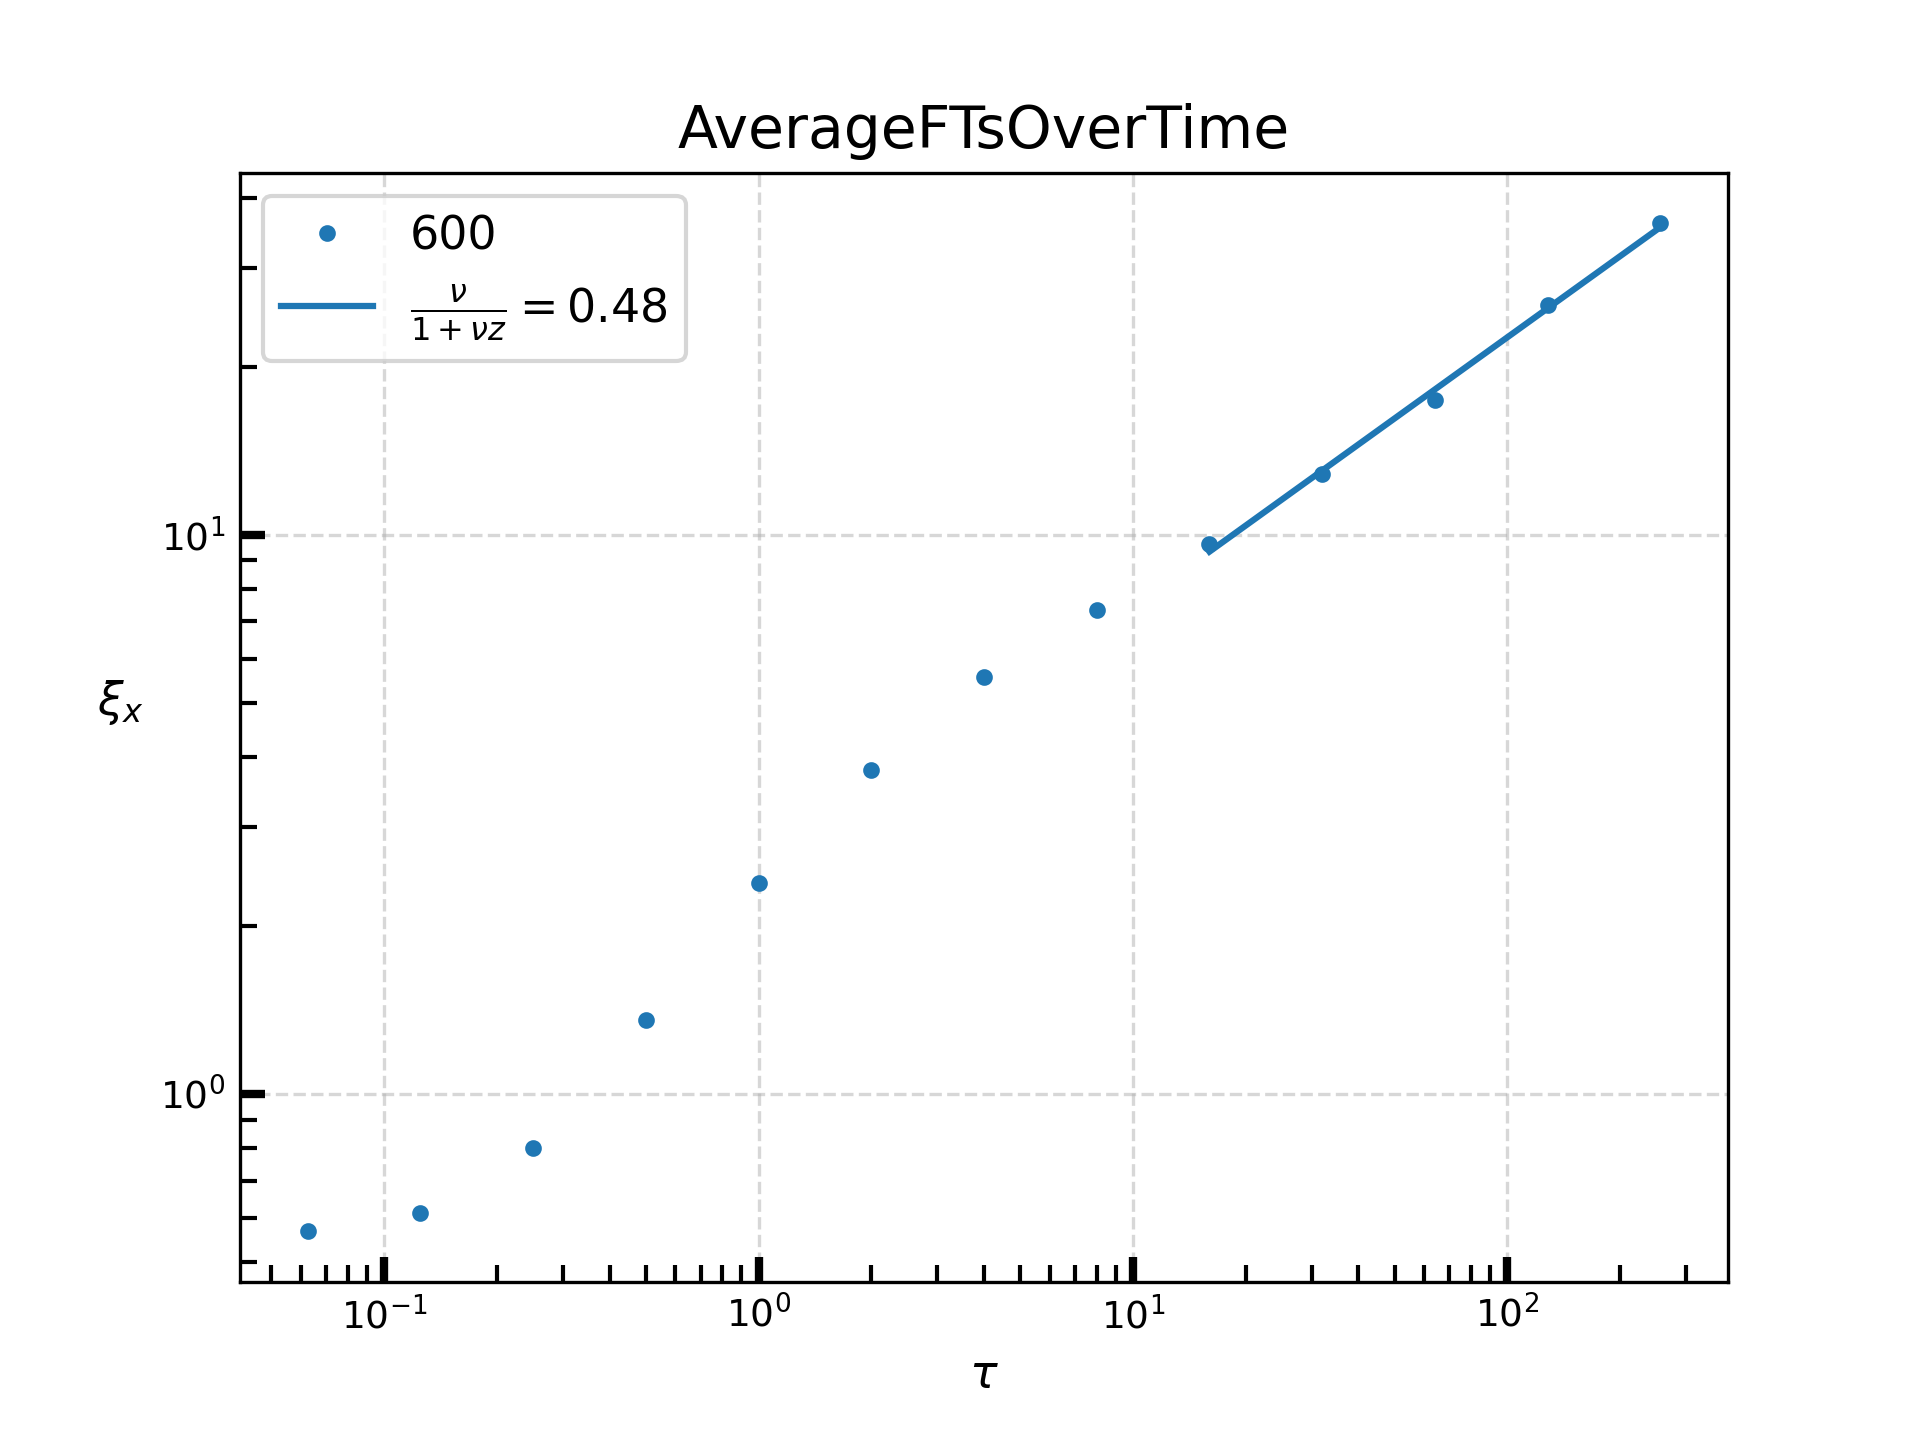
\includegraphics[width=0.8\linewidth]{graphics/xix-quench-scaling.png}
				\caption{The frozen correlation length $\hat{\xi}_x(\tau)$ depending on the quench timescale is investigated. A fit of the data to 
				\label{Fig::Quench-Resulb-c}
					\autoref{Eq::KZM-scaling} is calculated and drawn in the appropriate area.}
			\end{subfigure}
			\begin{subfigure}{0.5\textwidth}
				\centering
				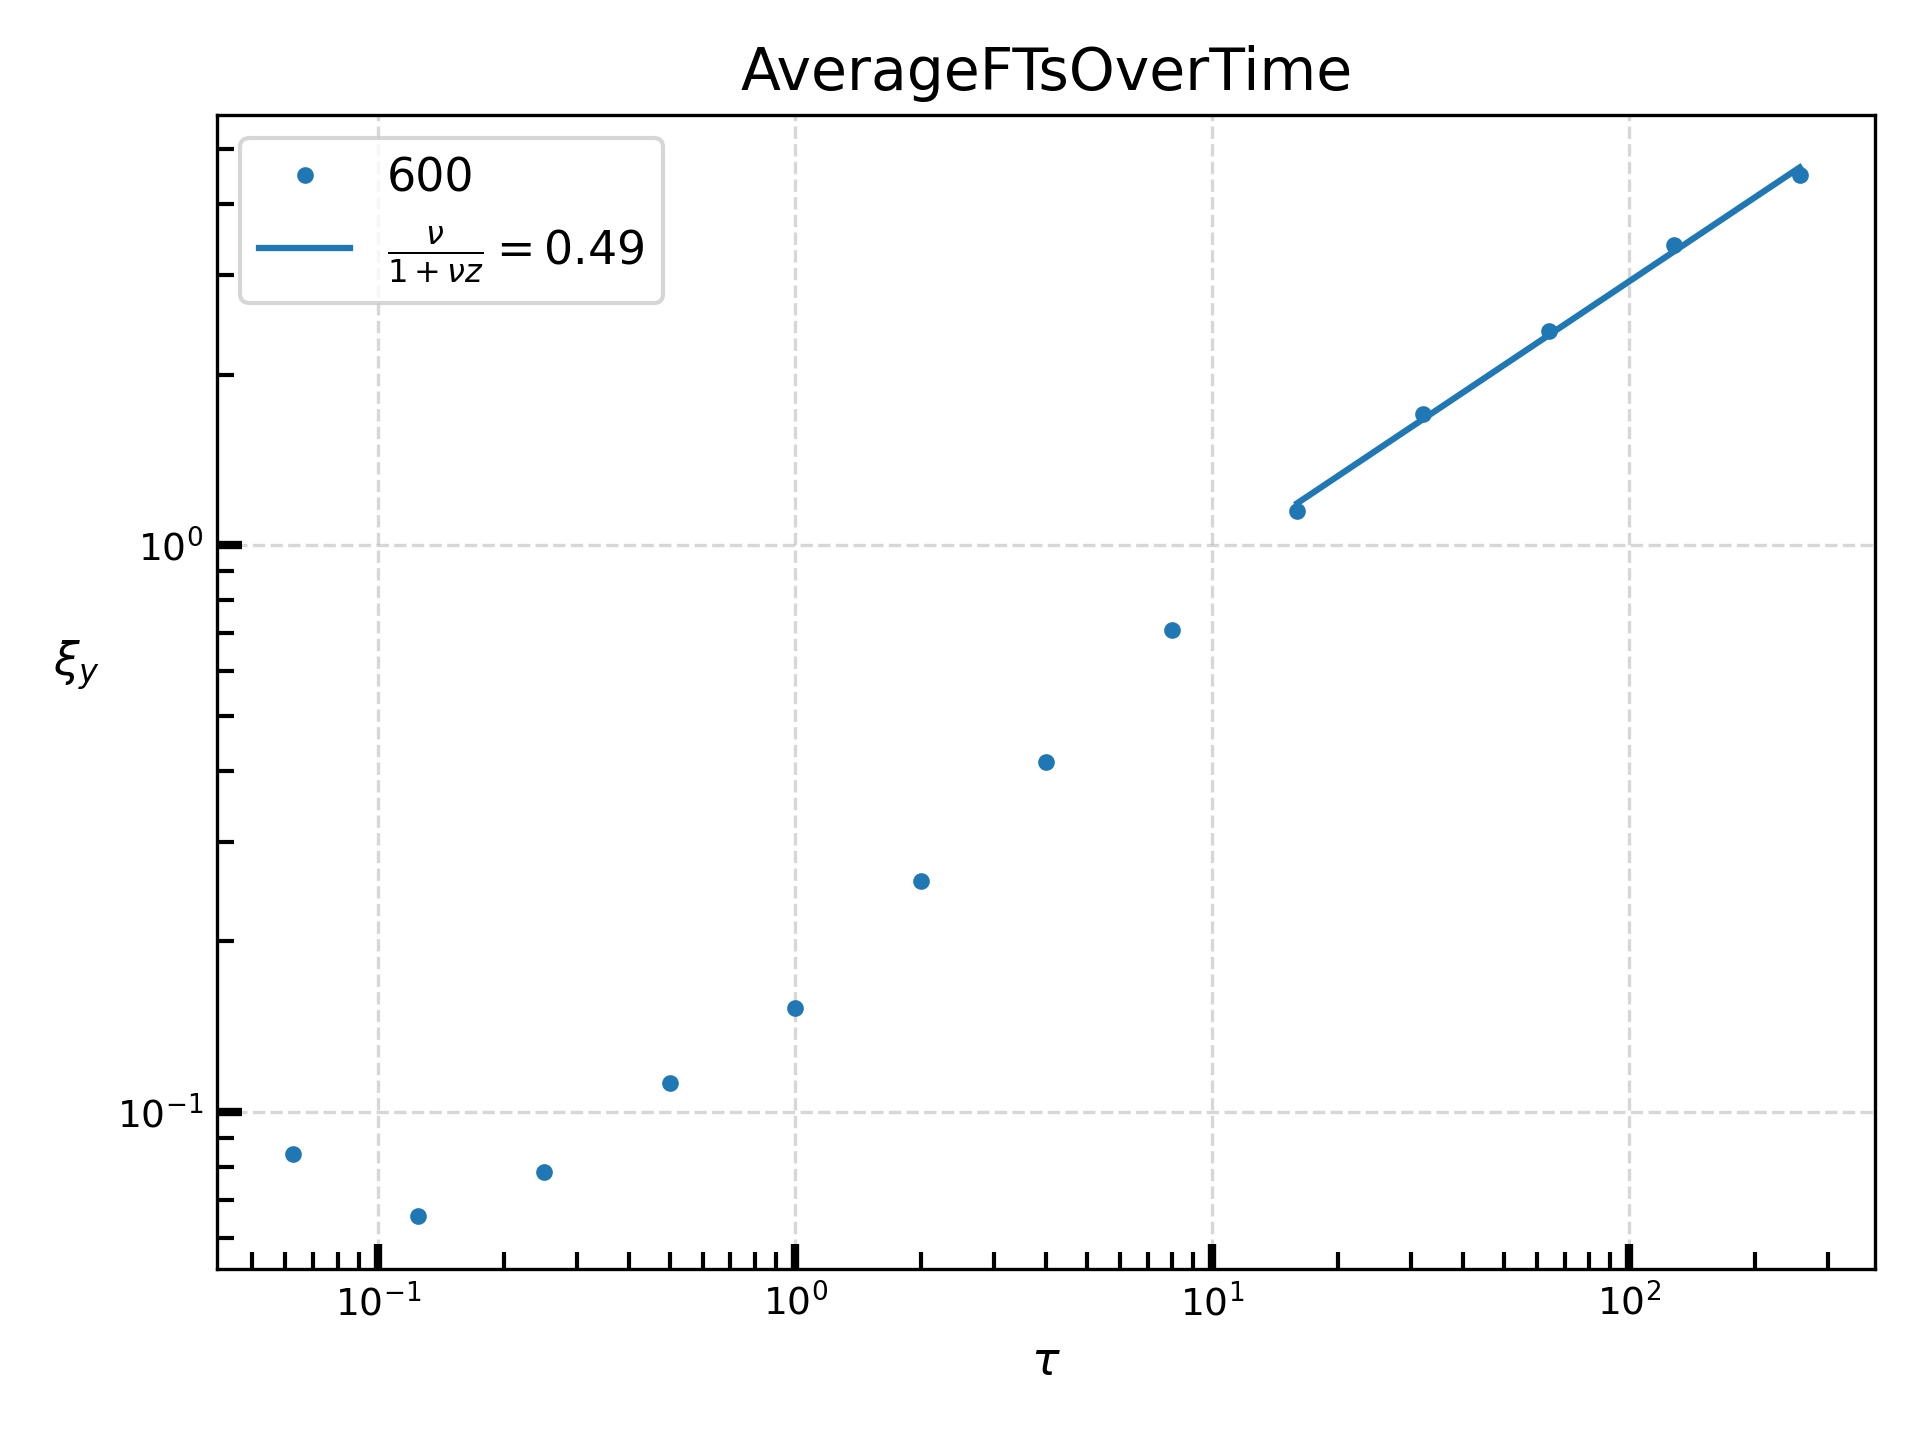
\includegraphics[width=0.8\linewidth]{graphics/xiy-quench-scaling.png}
				\caption{The frozen correlation length $\hat{\xi}_y(\tau)$ depending on the quench timescale is investigated. A fit of the data to \autoref{Eq::KZM-scaling} is calculated and drawn in the appropriate area.}
				\label{Fig::Quench-Resulb-d}
			\end{subfigure}
			\caption{The results of the quenches are investigated using the Kibble Zurek mechanism. The Kibble-Zurek mechanism is valid where the system is at the start of the quench able to adiabatically follow the process. When the quench is so fast that the system cannot follow the quench even at the start, the frozen correlation length is the equilibrium correlation length of the starting temperature and no scaling is observed.}
			\label{Fig::Quench-Result}
		\end{figure}  
		\subsubsection{Relaxation of the Binder cumulant}
		A simple way to examine the dynamic critical exponent is to consider the relaxation of the Binder cumulant including finite size scaling. This method was introduced by Li et. al \cite{li1995dynamic} and will be used in the following to extract the dynamic critical exponent. \\
		
		The basis is the time-resolved finite size scaling of the $(n)-$th moment of the magnetization
		\begin{equation} \label{Eq::Dynamic-FSS-M}
			M^{(n)}(t, \varepsilon, L) = b^{-n \beta / \nu} M^{(n)}(b^{-z}t, b^{1 /	\nu} \tau, b^{-1} L) ~,
		\end{equation}
		with $b =	\tfrac{L}{L'}$ being the spatial rescaling factor. Janssen et. al \cite{janssen1989new} determined that the initial correlation length must be very short for \autoref{Eq::Dynamic-FSS-M} to be valid. Therefore the investigated systems will be prepared in a high temperature, low order state.
		Following the definition of the Binder cumulant  \autoref{Eq::Def-Binder-Cum}, one can relate the Binder cumulant of systems of different sizes at the critical point $\varepsilon =	0$ by
		\begin{equation}
			U(t, 0, L_1) =	U(b^{-z} t, 0, L_2)~, \qquad \text{with} \qquad b = \frac{L_1}{L_2}
		\end{equation}
		The exponent $z$ is easily obtained by searching a time rescaling factor $b^{-z}$ such that the recorded curves for $U_{L_1}$ and $U_{L_2}$ collapse. Since the sample systems are prepared in a high temperature state where $U_L =	3$, we expect a relaxation from this value to the equilibrium $U_L^*$ which is, at $\varepsilon =	0$, the same for every system size. 
		\begin{figure}[htp]
			\centering
			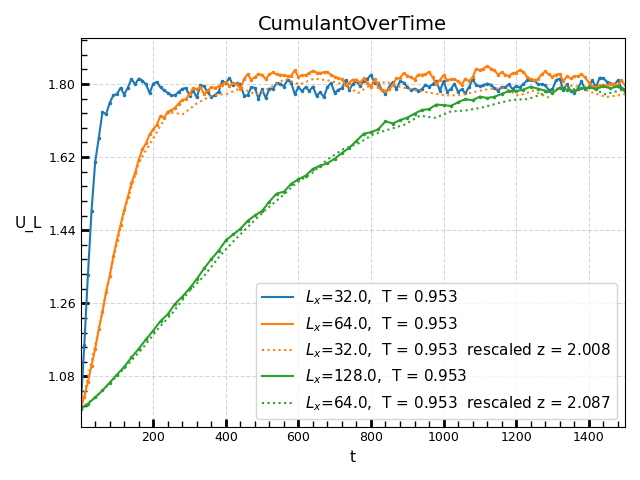
\includegraphics[width=0.8\linewidth]{graphics/cum-over-time-scan.png}
			\caption{The best rescaling of $U_{L_1} \rightarrow U_{L_2}$ is selected by minimizing the squared error between the interpolated curves. The result of the rescaling from $64 \rightarrow 128$ yields a dynamic critical exponent of $z = 2.08$, close to the best known value for the Ising universality class (see \autoref{Table::Ising-crit-expo}). }
			\label{Fig::Cum-Relax-z-extrac}
		\end{figure}
		The results for the rescalings $32 \rightarrow 64$ and $64 \rightarrow 128$ calculated from ??? sample paths are shown in \autoref{Fig::Cum-Relax-z-extrac}. The rescaling $64 \rightarrow 128$ is to be trusted more than the $32 \rightarrow 64$ since it minimizes the finite size corrections to the scaling law \autoref{Eq::Dynamic-FSS-M}. Its result $z =	2.08$ is very close to the best available dynamical critical exponent of the Ising model $z_{Ising}=2.14$.With this the calculated KZM exponent of $\nu /	(1 + z\nu) = 0.33	$ stands in harsh contradiction to the exponent obtained directly from the quench $\nu /	(1 + z\nu) = 0.45$. Since it is from symmetry considerations very plausible that our model for silicon would show the Ising dynamical exponent, we would expect that the deviation stems from the Kibble-Zurek scaling. Since the system sizes used in the quenches is already very large, strong finite size corrections to the Kibble-Zurek scaling can be ruled out as cause of the deviation. The same is true for the discretization error of our stepsize since the same quenches have been recalculated with a smaller stepsize. Since the correctness of our simulation has otherwise been verified, the most sensible explanation for the large Kibble-Zurek scaling exponent is that the cause has to be a systematic difference in the expected Kibble-Zurek mechanics (???). An idea could be the existence of subleading scalings like reported in \cite{ladewig2020kibble} caused by other scaling fields than the temperature. In our case such a scaling field could be the strength of the external potential $h$. \\
		
		In the following we will investigate the effect of the strength of $h$ on the dynamical critical exponent as well as the Kibble-Zurek exponent.

		\subsection{other}
		\subsection{quantitative?}
	\section{Discussion}
\chapter{Summary and Lookout}
	\section{Summary}
	\section{Lookout}
	\newpage
	\begin{equation*}
		\vartheta
	\end{equation*}

	\begin{equation*}
		\varphi
	\end{equation*}

	\begin{equation*}
		\phi
	\end{equation*}
		
	\appendix
	\chapter{Appendix}	
	\section{Caldeira-Legget calculation} \label{Section::Appendix-Caldeira-Legget}
	Starting point for this calculation is \autoref{Eq::Caldeira-Legget-Startpoint}. Consider the trace in the second term in \autoref{Eq::Caldeira-Legget-Startpoint}:
	\begin{equation}
		\text{tr}_B \left\{  \left[{\hat{H}}_I, \left[{\boldsymbol{\hat{H}}}_I(- \tau), {\hat{\rho}}_S(t) \otimes \overline{\rho}_B \right]\right]  \right\} =	\text{tr}_B \left\{  \left[\hat{x} \otimes \hat{B}, \left[{\boldsymbol{\hat{x}}}(- \tau) \otimes \boldsymbol{\hat{B}}(- \tau), {\hat{\rho}}_S(t) \otimes \overline{\rho}_B \right]\right]  \right\}~.
	\end{equation}
	Multiplying out the commutator yields
	\begin{equation} \label{Eq::Caldeira-Leggett-Trace}
		\begin{split}
			(\text{A.1})~=\text{tr}_B \bigg \{+&\hat{x} \boldsymbol{\hat{x}}(-\tau) \hat{\rho}_S(t) \otimes \hat{B} \boldsymbol{\hat{B}}(-\tau) \overline{\rho}_B 
			- \hat{x}  \hat{\rho}_S(t) \boldsymbol{\hat{x}}(-\tau) \otimes \hat{B}  ~\overline{\rho}_B \boldsymbol{\hat{B}}(-\tau)\\
			-&  \boldsymbol{\hat{x}}(-\tau) \hat{\rho}_S(t) \hat{x} \otimes  	\boldsymbol{\hat{B}}(-\tau) \overline{\rho}_B \hat{B}
			+ \hat{\rho}_S(t) \hat{x} \boldsymbol{\hat{x}}(-\tau)  \otimes \overline{\rho}_B \boldsymbol{\hat{B}}(-\tau) \hat{B}   \bigg \}~.
		\end{split}
	\end{equation}
	The factors belonging to the Hilbert space of the system can be pulled out of the trace. Additionally we use the cyclic property of the trace as well as the expectation value representation $\left \langle \hat{A} \right \rangle =	\text{tr}\left(\hat{A}\rho\right)$ to obtain
	\begin{equation}
		\begin{split}
			(\text{A}.2) =	~~  &\Big (\hat{x} \boldsymbol{\hat{x}}(-\tau) \hat{\rho}_S(t) - \boldsymbol{\hat{x}}(-\tau) \hat{\rho}_S(t) \hat{x}   \Big) \left \langle \hat{B} \boldsymbol{\hat{B}}(-\tau) \right \rangle \\
			+& \Big (  \hat{\rho}_S(t) \boldsymbol{\hat{x}}(-\tau) \hat{x}  - \hat{x} \hat{\rho}_S(t) \boldsymbol{\hat{x}}(-\tau)    \Big) \left \langle \boldsymbol{\hat{B}}(-\tau) \hat{B}  \right \rangle ~.
		\end{split}
	\end{equation}
	We can rewrite $\langle \hat{B} \boldsymbol{\hat{B}}(-\tau) \rangle = \frac{1}{2}	\langle [\hat{B}, \boldsymbol{\hat{B}}(-\tau)] + \{ \hat{B},  \boldsymbol{\hat{B}}(-\tau)\} \rangle$ and likewise $ \langle \boldsymbol{\hat{B}}(-\tau) \hat{B}  \rangle$ which yields
	\begin{equation} \label{Eq::Expanded-Bath-Operators}
		\begin{split}
			\text{(A.3)} =	&\frac{1}{2} \left\langle \left[\hat{B}, \boldsymbol{\hat{B}}(-\tau) \right]  \right \rangle \Big ( +\hat{x} \boldsymbol{\hat{x}}(-\tau) \hat{\rho}_S(t) + \hat{x} \hat{\rho}_S(t) \boldsymbol{\hat{x}}(-\tau) - \boldsymbol{\hat{x}}(-\tau) \hat{\rho}_S(t) \hat{x}  \\
			& \qquad \qquad \qquad \qquad -  \hat{\rho}_S(t) \boldsymbol{\hat{x}}(-\tau) \hat{x} \Big ) \\
			& \frac{1}{2} \left\langle \left \{\hat{B}, \boldsymbol{\hat{B}}(-\tau)\right \}  \right \rangle \Big ( \hat{x} \boldsymbol{\hat{x}}(-\tau) \hat{\rho}_S(t) - \hat{x} \hat{\rho}_S(t) \boldsymbol{\hat{x}}(-\tau) - \boldsymbol{\hat{x}}(-\tau) \hat{\rho}_S(t) \hat{x} \\
			& \qquad \qquad \qquad \qquad + \hat{\rho}_S(t) \boldsymbol{\hat{x}}(-\tau) \hat{x} \Big) ~.
		\end{split}
	\end{equation}
	The position operator terms can be combined to
	\begin{align} \label{Eq::recombined-pos-operators}
		&\left[\hat{x}, \left\{\boldsymbol{\hat{x}}(-\tau),  \hat{\rho}_S(t)\right\}\right] =	\hat{x} \boldsymbol{\hat{x}}(-\tau) \hat{\rho}_S(t) + \hat{x} \hat{\rho}_S(t) \boldsymbol{\hat{x}}(-\tau) - \boldsymbol{\hat{x}}(-\tau) \hat{\rho}_S(t) \hat{x}
		-  \hat{\rho}_S(t) \boldsymbol{\hat{x}}(-\tau) \hat{x} \\
		&\left[\hat{x}, \left[\boldsymbol{\hat{x}}(-\tau),  \hat{\rho}_S(t)\right] \right] =	\hat{x} \boldsymbol{\hat{x}}(-\tau) \hat{\rho}_S(t) - \hat{x} \hat{\rho}_S(t) \boldsymbol{\hat{x}}(-\tau) - \boldsymbol{\hat{x}}(-\tau) \hat{\rho}_S(t) \hat{x}
		+  \hat{\rho}_S(t) \boldsymbol{\hat{x}}(-\tau) \hat{x}~.
	\end{align}
	Plugging \autoref{Eq::recombined-pos-operators} into \autoref{Eq::Expanded-Bath-Operators} yields for the trace of \autoref{Eq::Caldeira-Leggett-Trace}:
	\begin{equation}
		\begin{split}
			\text{tr}_B \left\{  \left[{\hat{H}}_I, \left[{\boldsymbol{\hat{H}}}_I(- \tau), {\hat{\rho}}_S(t) \otimes \overline{\rho}_B \right]\right]  \right\} =	~&\frac{1}{2} \left\langle \left[\hat{B}, \boldsymbol{\hat{B}}(-\tau) \right]  \right \rangle \left[\hat{x}, \left\{\boldsymbol{\hat{x}}(-\tau),  \hat{\rho}_S(t)\right\}\right] \\
			& \frac{1}{2} \left\langle \left \{\hat{B}, \boldsymbol{\hat{B}}(-\tau)\right \}  \right \rangle \left[\hat{x}, \left[\boldsymbol{\hat{x}}(-\tau),  \hat{\rho}_S(t)\right] \right]
		\end{split}
	\end{equation}
	We will now try to find expressions for $\langle [\hat{B}, \boldsymbol{\hat{B}}(-\tau) ]  \rangle$ and $\langle  \{\hat{B}, \boldsymbol{\hat{B}}(-\tau) \}  \rangle$. The interaction picture operator $\boldsymbol{\hat{B}}(-\tau)$ can be calculated by it's definition
	\begin{equation}
		\begin{split}
			\boldsymbol{\hat{B}}(-\tau) =	e^{i \hat{H}_B (-\tau)} \hat{B} e^{- i \hat{H}_B (-\tau)} &=	 e^{i \hat{H}_B (-\tau)} \sum_n \kappa_n \sqrt{\frac{\hbar}{2 m_n \omega_n}} \left(\hat{b}_n + \hat{b}_n^\dagger\right) e^{- i \hat{H}_B (-\tau)} \\
			&=	\sum_n \kappa_n \sqrt{\frac{\hbar}{2 m_n \omega_n}} \left(\boldsymbol{\hat{b}}_n(-\tau) + \boldsymbol{\hat{b}}_n^\dagger(-\tau) \right)~.		
		\end{split}	
	\end{equation}
	For the transformation of the bosonic creation and annihilation operators one can derive a differential equation
	\begin{equation} \label{Eq::creation-annihilation-ode}
		\begin{split}
			\frac{\text{d}}{\text{dt}} \boldsymbol{\hat{b}}^{(\dagger)}_n(-\tau) &=	\frac{\text{d}}{\text{dt}} \left(e^{- i \hat{H}_B \tau}~ \hat{b}_n^{(\dagger)}~e^{ i \hat{H}_B \tau}\right) = -i~e^{- i \hat{H}_B \tau}~ \left[\hat{H}_B, \hat{b}_n^{(\dagger)}\right]~e^{i \hat{H}_B \tau} \\
			&=	(-)i~e^{- i \hat{H}_B \tau}~ \hat{b}_n^{(\dagger)}~e^{i \hat{H}_B \tau}  =	(-)i\omega_n \boldsymbol{\hat{b}}_n^{(\dagger)}~,
		\end{split}		
	\end{equation}
	and solve it under the initial condition $\boldsymbol{\hat{b}}_n^{(\dagger)}(0) = \hat{b}_n^{(\dagger)}	$. The solution to \autoref{Eq::creation-annihilation-ode} is
	\begin{equation}
		\boldsymbol{\hat{b}}_n^{(\dagger)}(-\tau) = \hat{b}_n^{(\dagger)} e^{(-)i\omega_n \tau}~,
	\end{equation}
	leading to 
	\begin{equation}
		\boldsymbol{\hat{B}}(-\tau) =	\sum_n \kappa_n \sqrt{\frac{\hbar}{2 m_n \omega_n}} \left({\hat{b}_n}e^{i \omega \tau} + {\hat{b}_n}^\dagger e^{-i \omega_n \tau} \right)~.
	\end{equation}
	Now we can calculate the commutator $[\hat{B}, \boldsymbol{\hat{B}}(-\tau) ]$:
	\begin{equation} \label{Eq::Bath-commutator-calculation}
		\begin{split}
			\left[\hat{B}, \boldsymbol{\hat{B}}(-\tau) \right] &=	\sum_{n,k}^{} \frac{\kappa_n \kappa_k}{2 \sqrt{\omega_n \omega_k}} \left[\hat{b}_n^\dagger + \hat{b}_n , {\hat{b}_k}e^{i \omega_k \tau} + {\hat{b}_k}^\dagger e^{-i \omega_k \tau} \right] \\
			&= \sum_{n,k}^{} \frac{\kappa_n \kappa_k}{2 \sqrt{\omega_n \omega_k}} \left\{\left[\hat{b}_n^\dagger, \hat{b}_k\right] e^{i\omega_k \tau} + \left[\hat{b}_n, \hat{b}_k^\dagger\right] e^{-i\omega_k \tau}\right\} \\
			&= \sum_{n,k}^{} \frac{\kappa_n \kappa_k}{2 \sqrt{\omega_n \omega_k}} \left\{\delta_{nk} e^{-i\omega_k \tau} - \delta_{nk} e^{i\omega_k \tau}\right\} \\
			&= \sum_{n}^{} \frac{\kappa_n^2 }{2 {\omega_n^2}} \left\{e^{-i\omega_k \tau} - e^{i\omega_k \tau}\right\} \\
			&= - 2 i  \sum_{n}^{} \frac{\kappa_n^2 }{2 {\omega_n^2}} \sin \omega_n \tau 
		\end{split}
	\end{equation}
	Since this is a constant $\langle [\hat{B}, \boldsymbol{\hat{B}}(-\tau) ]  \rangle =	[\hat{B}, \boldsymbol{\hat{B}}(-\tau) ]$. By introducing the reservoir spectral density 
	\begin{equation}
		J(\omega) =	\sum_n =	\frac{\kappa_n^2}{2 \omega_n} \delta(\omega - \omega_n)~,
	\end{equation}
	\autoref{Eq::Bath-commutator-calculation} may be written as an integral
	\begin{equation}
		\left\langle \left[\hat{B}, \boldsymbol{\hat{B}}(-\tau) \right] \right \rangle = -2i \int_{0}^{\infty} d\omega J(\omega) \sin \omega \tau~.
	\end{equation}
	Under Born approximation, the reservoir is in thermal equilibrium so that the density matrix can be written as
	\begin{equation}
		\overline{\rho}_B =	\frac{e^{-\beta H_B}}{\text{tr}\left(e^{-\beta H_B}\right)}=\frac{1}{Z} e^{-\beta H_B}~.
	\end{equation}
	\section{Correlation Length calculation} \label{Section::Corr-Lenght-Calculation}
	TODO
	\bibliographystyle{plain}
	\bibliography{references.bib}
	
% Erklärung
\clearpage
\thispagestyle{empty}
\minisec{Erklärung}\vspace*{1.5em}

Hiermit erkläre ich, dass ich diese Arbeit im Rahmen der Betreuung am Institut
für ??? Physik ohne unzulässige Hilfe Dritter verfasst und alle Quellen als solche gekennzeichnet habe.

\vspace*{45em}

Vorname Nachname \par
Dresden, Monat 2019

\end{document}
